\documentclass[11pt,letterpaper]{article}

\newenvironment{proof}{\noindent{\bf Proof:}}{\qed\bigskip}

\newtheorem{theorem}{Theorem}
\newtheorem{corollary}{Corollary}
\newtheorem{lemma}{Lemma} 
\newtheorem{claim}{Claim}
\newtheorem{fact}{Fact}
\newtheorem{definition}{Definition}
\newtheorem{assumption}{Assumption}
\newtheorem{observation}{Observation}
\newtheorem{example}{Example}
\newcommand{\qed}{\rule{7pt}{7pt}}

\newcommand{\solution}[4]{
\thispagestyle{plain} 
\newpage
\setcounter{page}{1}
\noindent
\begin{center}
\framebox{ \vbox{
\vspace{4mm}
\vspace{0.2in} 
{\centering \large\mbox{#3}}\\
\vspace{0.1in}
{#1 \hfill {Date: #2}}
}}
\end{center}
\markright{#1}
}

\newenvironment{algorithm}
{\begin{center}
\begin{tabular}{|l|}
\hline
\begin{minipage}{1in}
\begin{tabbing}
\quad\=\qquad\=\qquad\=\qquad\=\qquad\=\qquad\=\qquad\=\kill}
{\end{tabbing}
\end{minipage} \\
\hline
\end{tabular}
\end{center}}

\def\Comment#1{\textsf{\textsl{$\langle\!\langle$#1\/$\rangle\!\rangle$}}}



\usepackage{graphicx, amssymb, amsmath, listings, float, mathtools}
\usepackage{color, url}
\usepackage{romannum}
\usepackage{subcaption}
\usepackage{mwe}
\lstset{language = Python}
\lstset{breaklines}
\lstset{extendedchars=false}
 
\definecolor{codegreen}{rgb}{0,0.6,0}
\definecolor{codegray}{rgb}{0.5,0.5,0.5}
\definecolor{codepurple}{rgb}{0.58,0,0.82}
\definecolor{backcolour}{rgb}{0.95,0.95,0.92}
 
\lstdefinestyle{mystyle}{
    backgroundcolor=\color{backcolour},   
    commentstyle=\color{codegreen},
    keywordstyle=\color{magenta},
    numberstyle=\tiny\color{codegray},
    stringstyle=\color{codepurple},
    basicstyle=\footnotesize,
    breakatwhitespace=false,         
    breaklines=true,                 
    captionpos=b,                    
    keepspaces=true,                 
    numbers=left,                    
    numbersep=5pt,                  
    showspaces=false,                
    showstringspaces=false,
    showtabs=false,                  
    tabsize=2
}
 
\lstset{style=mystyle}

\oddsidemargin 0in
\evensidemargin 0in
\textwidth 6.5in
\topmargin -0.6in
\textheight 9.0in

\begin{document}
% -----------------------------------------------------------------------------
\solution{\large Jifu Zhao}{\large 12/15/2016}{\bf \Large IE 529 \hspace{0.5cm} 
		Fall 2016 \hspace{0.5cm} Computational Assignment 2}

% -----------------------------------------------------------------------------
\section*{\Large \Romannum{1}. Lloyd's (K-means)Algorithm}

\begin{description}

\item{1. }
In this part, the polynomial regression is conducted on the given dataset. The derivation is relatively simple, here we only give one simple version.

%  -----------------------------------------------------------------------------
\begin{figure}[htb]
        \centering
        \begin{subfigure}[b]{0.475\textwidth}
            \centering
            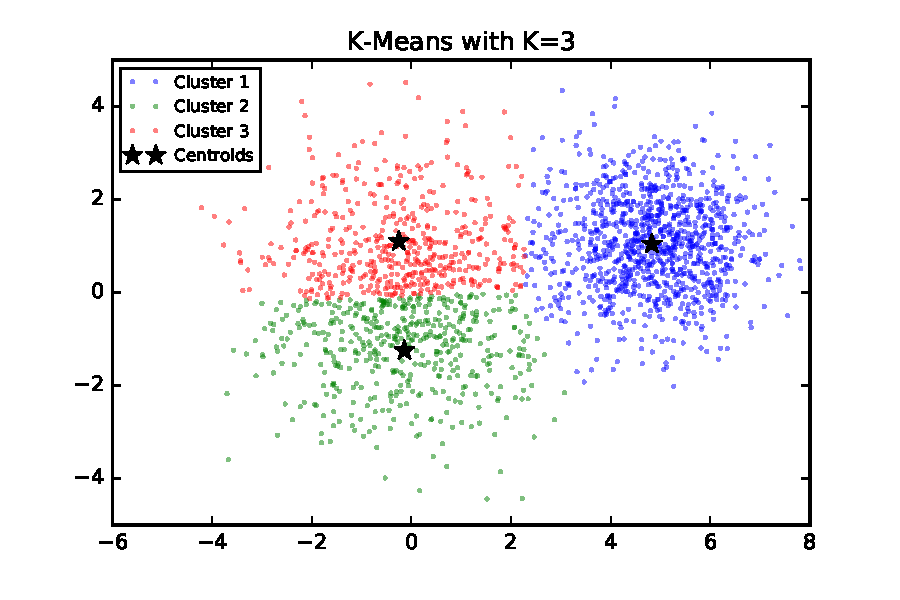
\includegraphics[width=\textwidth]{./figures/clustering_kMeans_3.pdf}
        \end{subfigure}
        \hfill
        \begin{subfigure}[b]{0.475\textwidth}  
            \centering 
            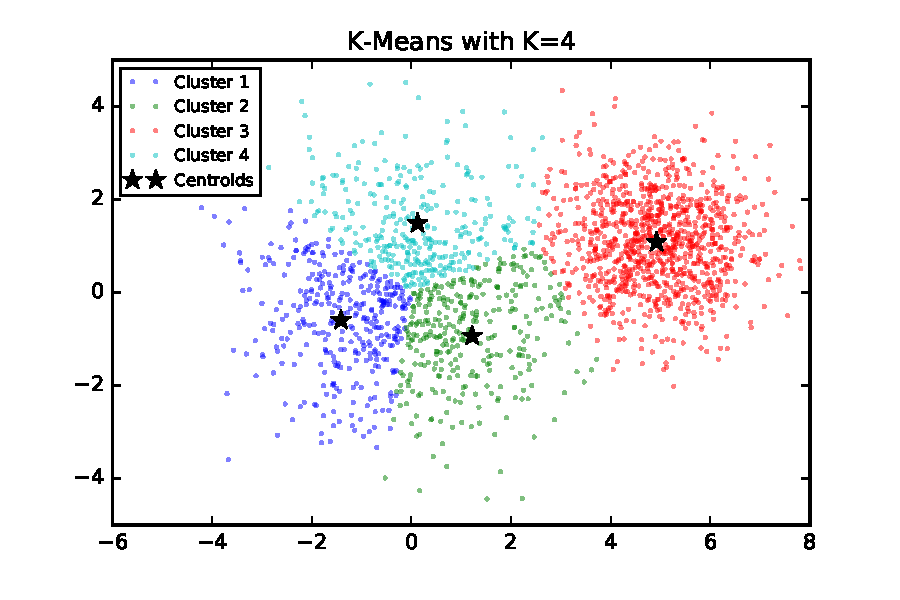
\includegraphics[width=\textwidth]{./figures/clustering_kMeans_4.pdf}
        \end{subfigure}
%        \vskip\baselineskip        
        \begin{subfigure}[b]{0.475\textwidth}  
            \centering 
            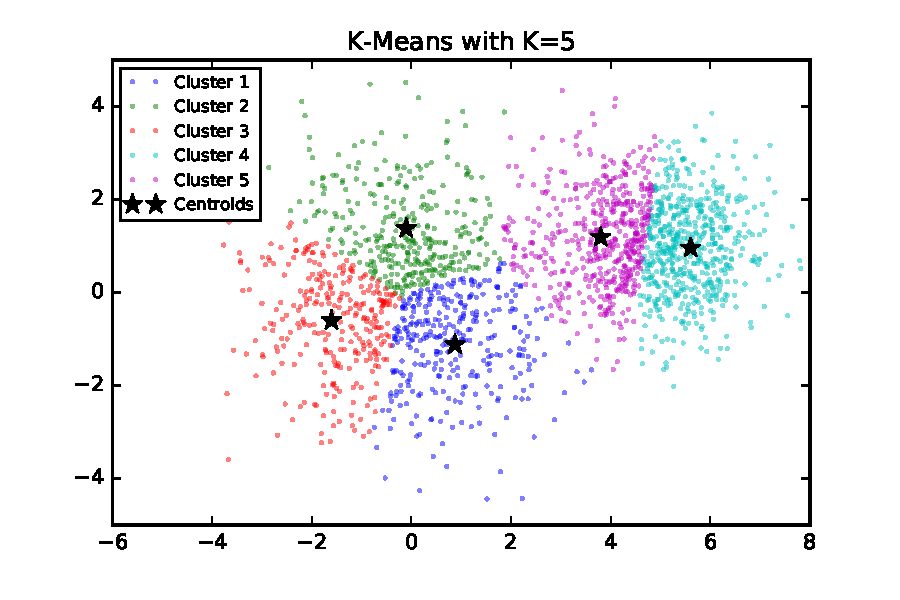
\includegraphics[width=\textwidth]{./figures/clustering_kMeans_5.pdf}
        \end{subfigure}
        \hfill
        \begin{subfigure}[b]{0.475\textwidth}   
            \centering 
            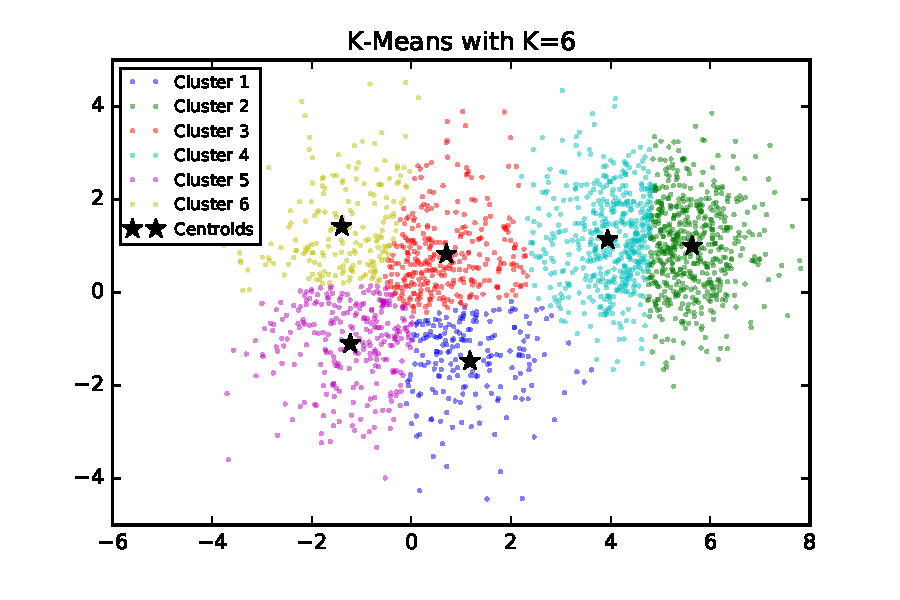
\includegraphics[width=\textwidth]{./figures/clustering_kMeans_6.pdf}
        \end{subfigure}
%        \vskip\baselineskip     
        \begin{subfigure}[b]{0.475\textwidth}   
            \centering 
            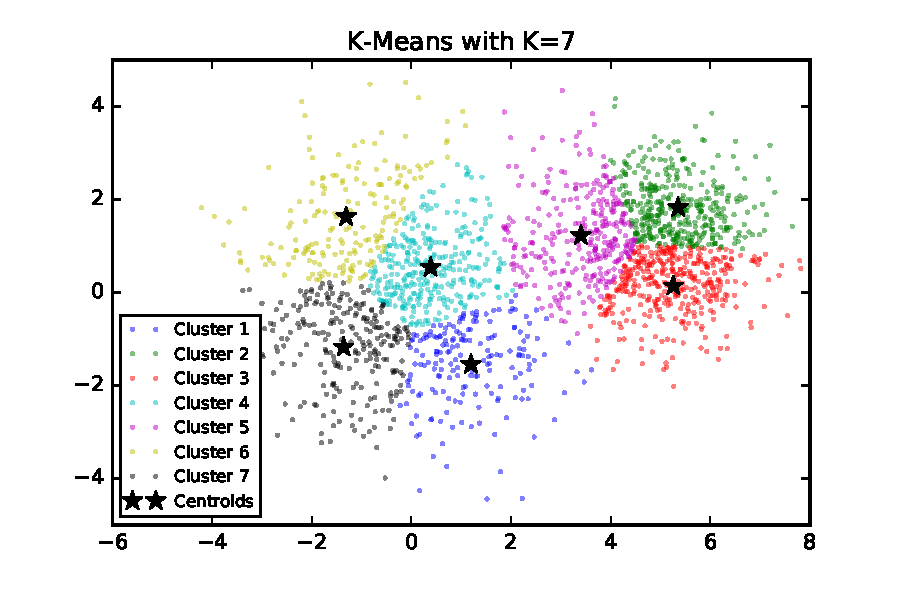
\includegraphics[width=\textwidth]{./figures/clustering_kMeans_7.pdf}
        \end{subfigure}
        \hfill
        \begin{subfigure}[b]{0.475\textwidth}  
            \centering 
            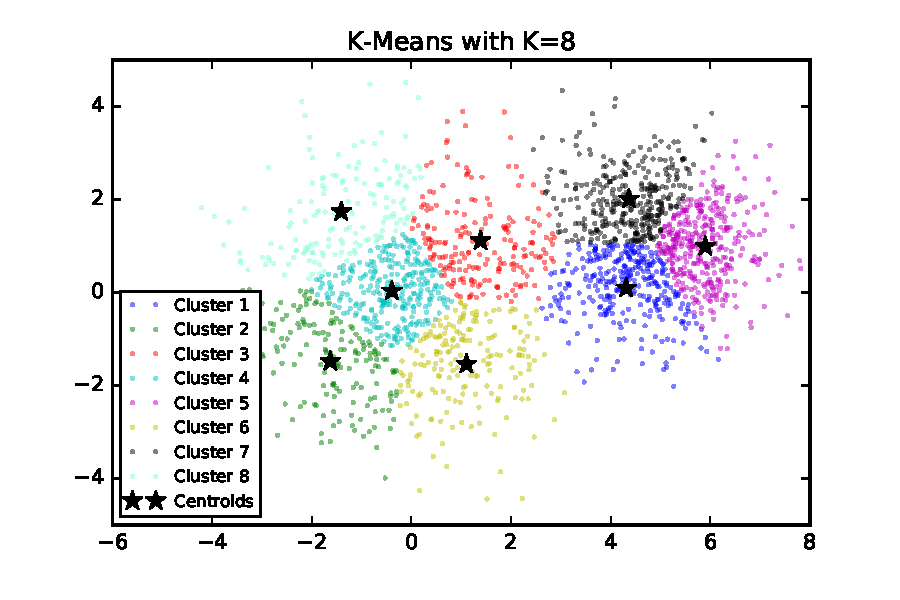
\includegraphics[width=\textwidth]{./figures/clustering_kMeans_8.pdf}
        \end{subfigure}
%        \vskip\baselineskip
        \begin{subfigure}[b]{0.475\textwidth}   
            \centering 
            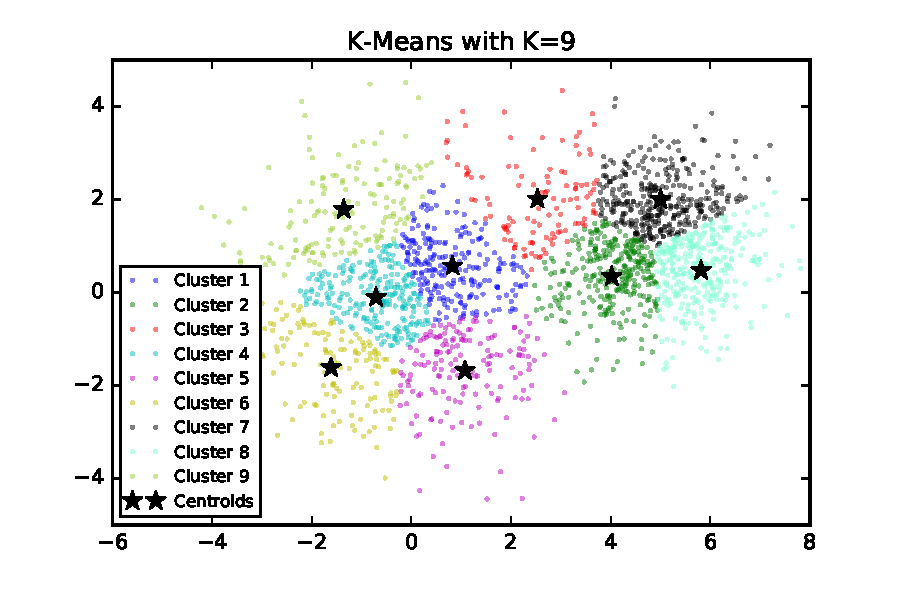
\includegraphics[width=\textwidth]{./figures/clustering_kMeans_9.pdf}
        \end{subfigure}
        \hfill
        \begin{subfigure}[b]{0.475\textwidth}   
            \centering 
            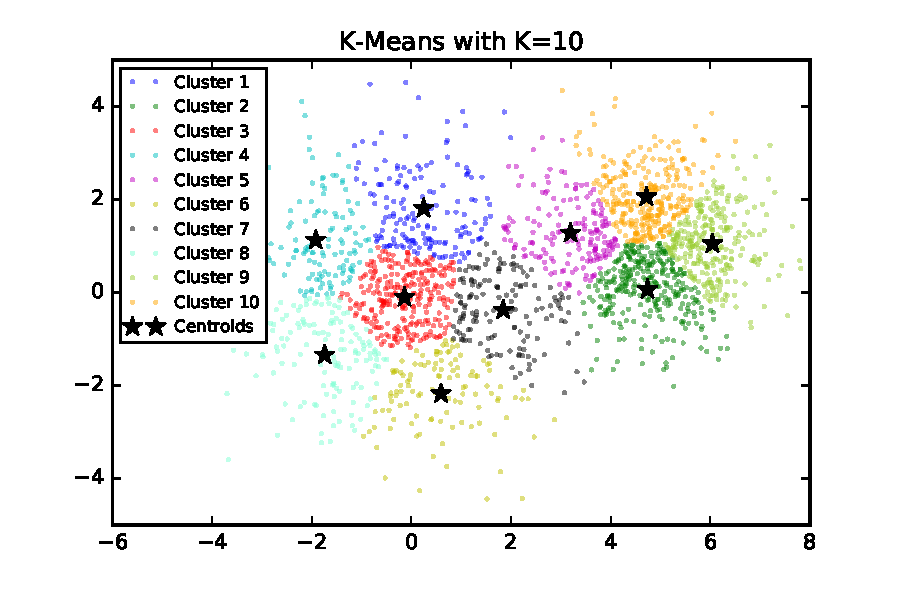
\includegraphics[width=\textwidth]{./figures/clustering_kMeans_10.pdf}
        \end{subfigure}
        
        \caption{Clustering Result for clustering.txt with K-Means Algorithm}
        \label{fig:kmean_clustering}
\end{figure}

%  -----------------------------------------------------------------------------
\begin{figure}[htb]
        \centering
        \begin{subfigure}[b]{0.475\textwidth}
            \centering
            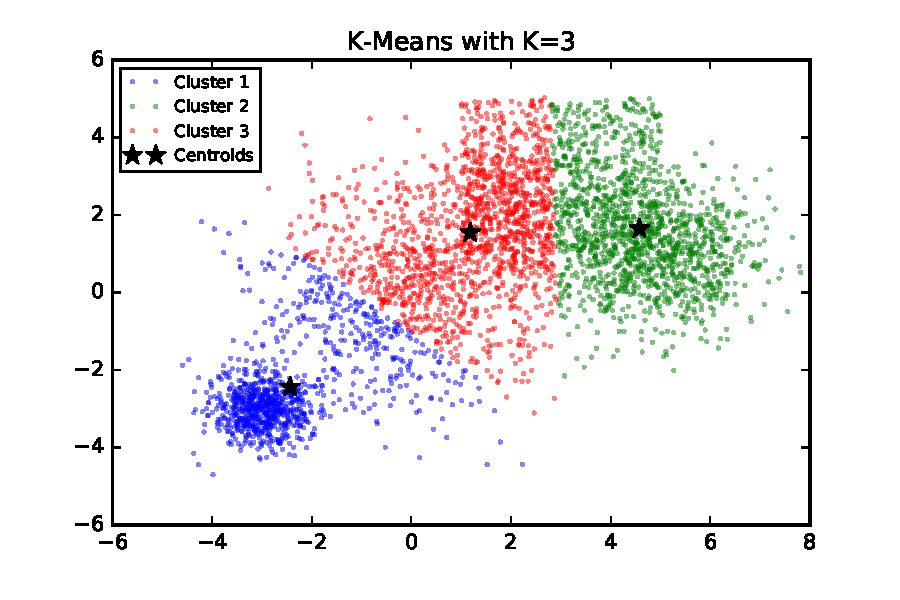
\includegraphics[width=\textwidth]{./figures/bigClustering_kMeans_3.pdf}
        \end{subfigure}
        \hfill
        \begin{subfigure}[b]{0.475\textwidth}  
            \centering 
            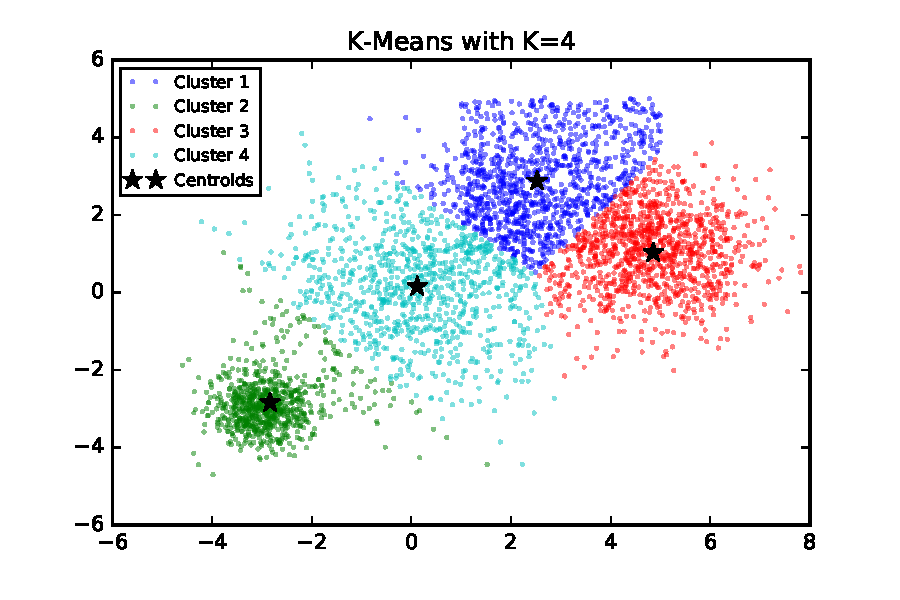
\includegraphics[width=\textwidth]{./figures/bigClustering_kMeans_4.pdf}
        \end{subfigure}
%        \vskip\baselineskip        
        \begin{subfigure}[b]{0.475\textwidth}  
            \centering 
            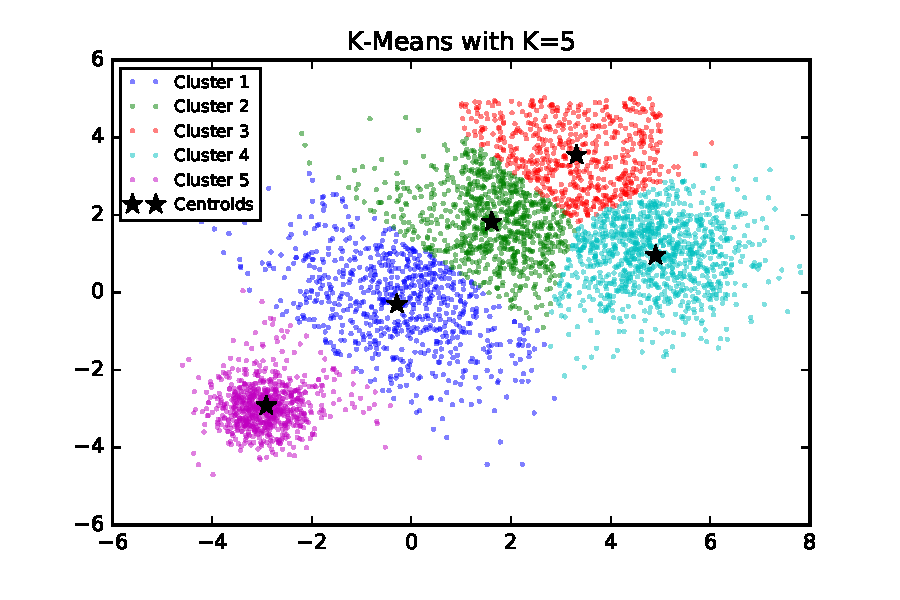
\includegraphics[width=\textwidth]{./figures/bigClustering_kMeans_5.pdf}
        \end{subfigure}
        \hfill
        \begin{subfigure}[b]{0.475\textwidth}   
            \centering 
            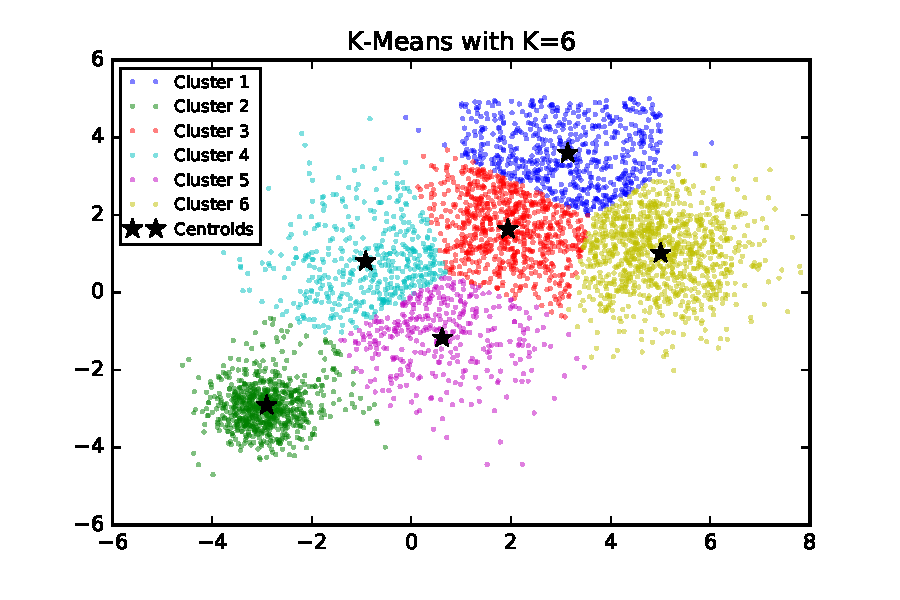
\includegraphics[width=\textwidth]{./figures/bigClustering_kMeans_6.pdf}
        \end{subfigure}
%        \vskip\baselineskip     
        \begin{subfigure}[b]{0.475\textwidth}   
            \centering 
            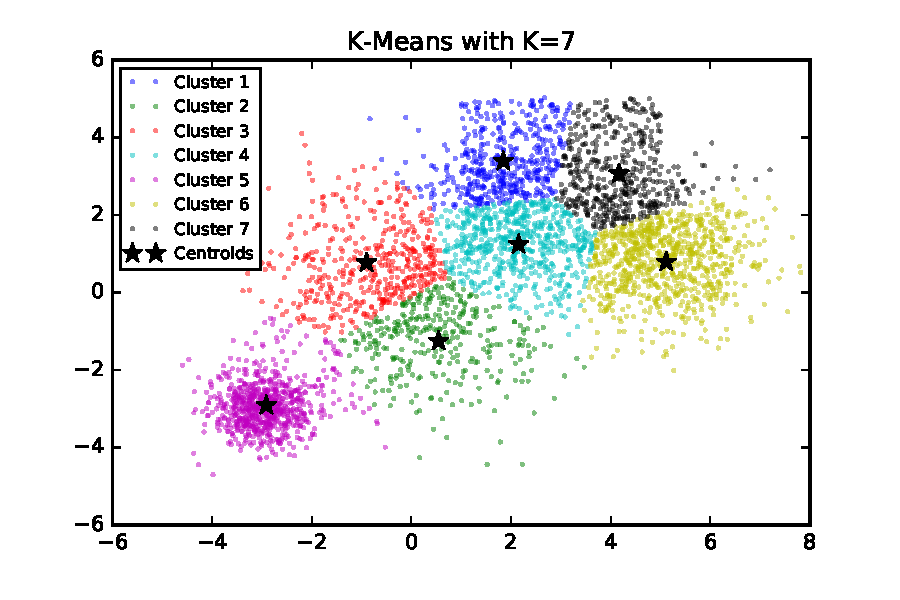
\includegraphics[width=\textwidth]{./figures/bigClustering_kMeans_7.pdf}
        \end{subfigure}
        \hfill
        \begin{subfigure}[b]{0.475\textwidth}  
            \centering 
            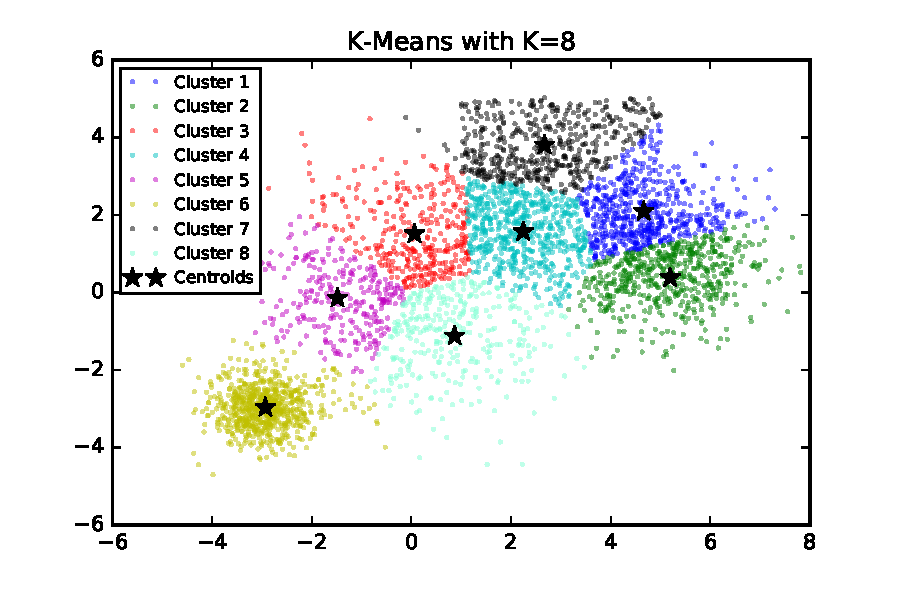
\includegraphics[width=\textwidth]{./figures/bigClustering_kMeans_8.pdf}
        \end{subfigure}
%        \vskip\baselineskip
        \begin{subfigure}[b]{0.475\textwidth}   
            \centering 
            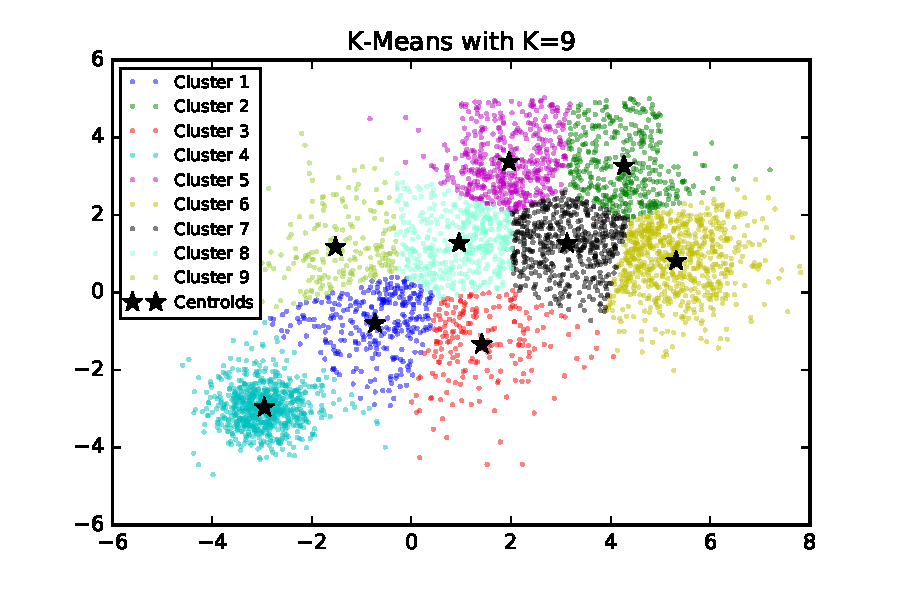
\includegraphics[width=\textwidth]{./figures/bigClustering_kMeans_9.pdf}
        \end{subfigure}
        \hfill
        \begin{subfigure}[b]{0.475\textwidth}   
            \centering 
            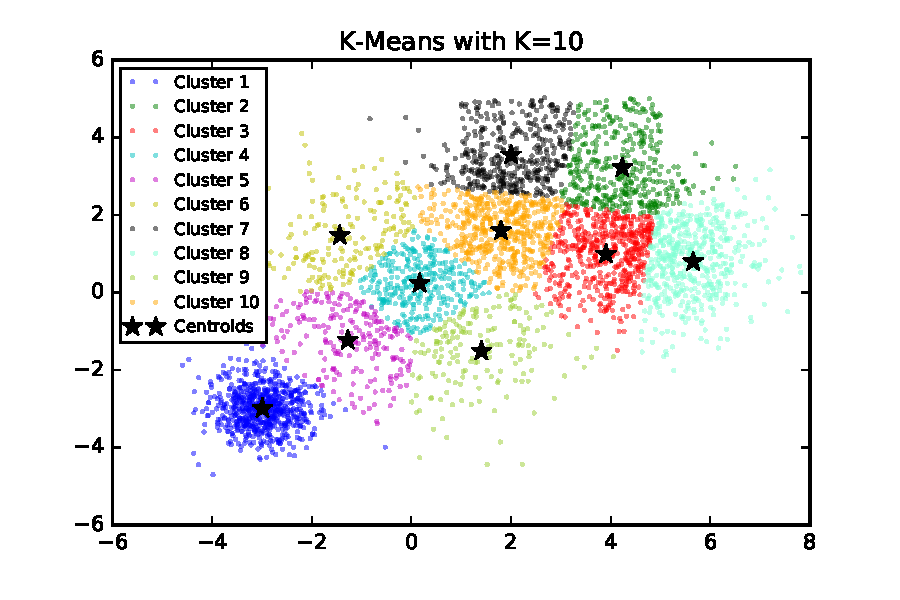
\includegraphics[width=\textwidth]{./figures/bigClustering_kMeans_10.pdf}
        \end{subfigure}
        
        \caption{Clustering Result for bigClusteringData.txt with K-Means Algorithm}
        \label{fig:kmean_clustering}
\end{figure}

%  -----------------------------------------------------------------------------
\begin{figure}[H]
\centering
\centering
        \begin{subfigure}[b]{0.49\textwidth}
            \centering
            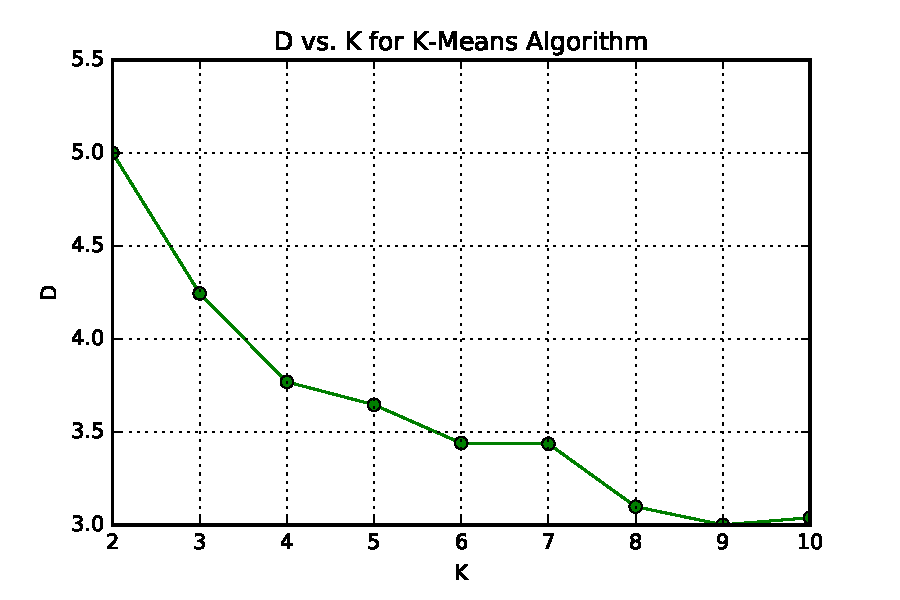
\includegraphics[width=\textwidth]{./figures/loss_clustering_kMeans.pdf}
            \caption{clustering.txt}\label{fig:3a}
        \end{subfigure}
        \hfill
        \begin{subfigure}[b]{0.49\textwidth}  
            \centering 
            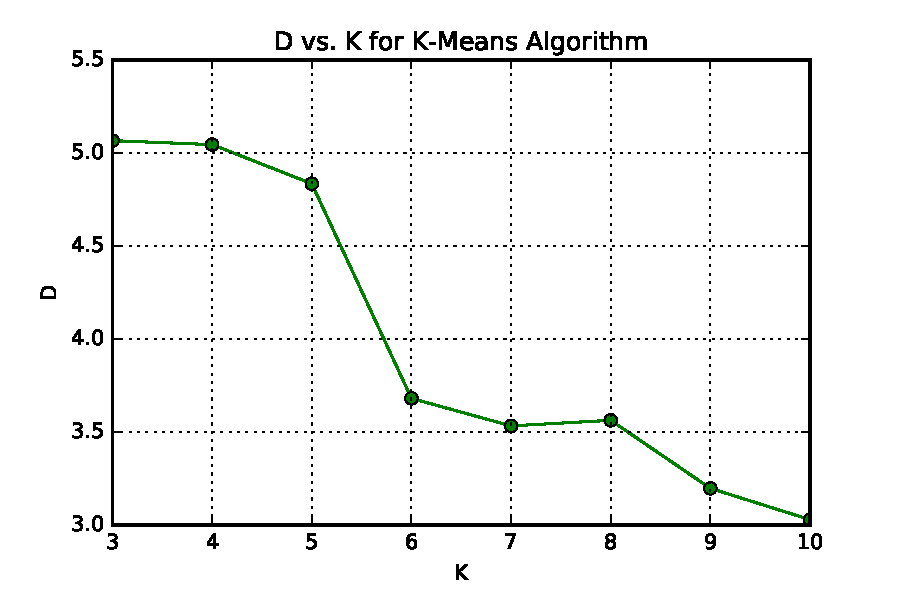
\includegraphics[width=\textwidth]{./figures/loss_bigClustering_kMeans.pdf}
            \caption{bigClusteringData.txt}\label{fig:3b}
        \end{subfigure}
\caption{Change of Distoration versus Cluster Number K for K-Means Algorithm}
\label{fig:k-means-loss} 
\end{figure}

\end{description}

% -----------------------------------------------------------------------------
\section*{\Large \Romannum{2}. Greedy K-centers Algorithm}

%  -----------------------------------------------------------------------------
\begin{figure}[htb]
        \centering
        \begin{subfigure}[b]{0.475\textwidth}
            \centering
            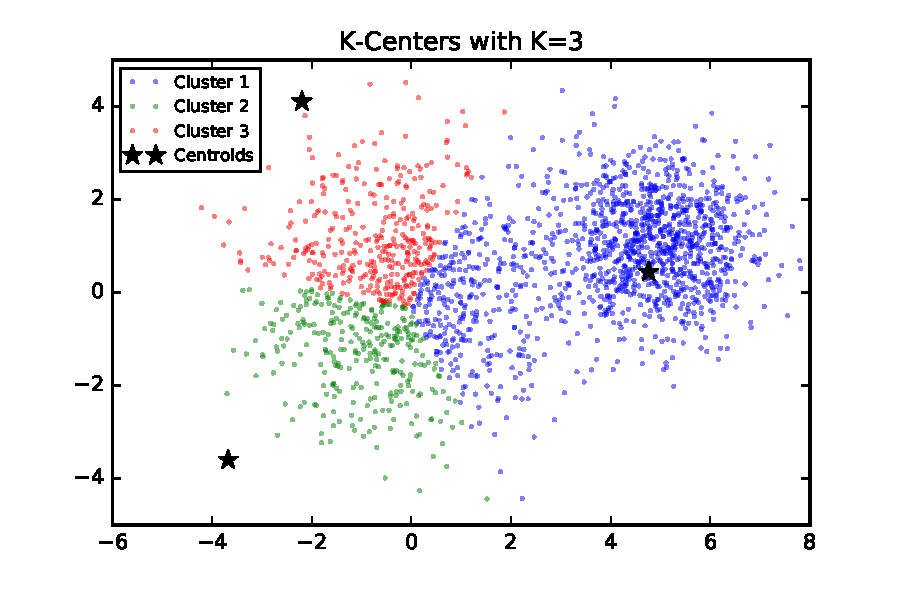
\includegraphics[width=\textwidth]{./figures/clustering_kCenter_3.pdf}
        \end{subfigure}
        \hfill
        \begin{subfigure}[b]{0.475\textwidth}  
            \centering 
            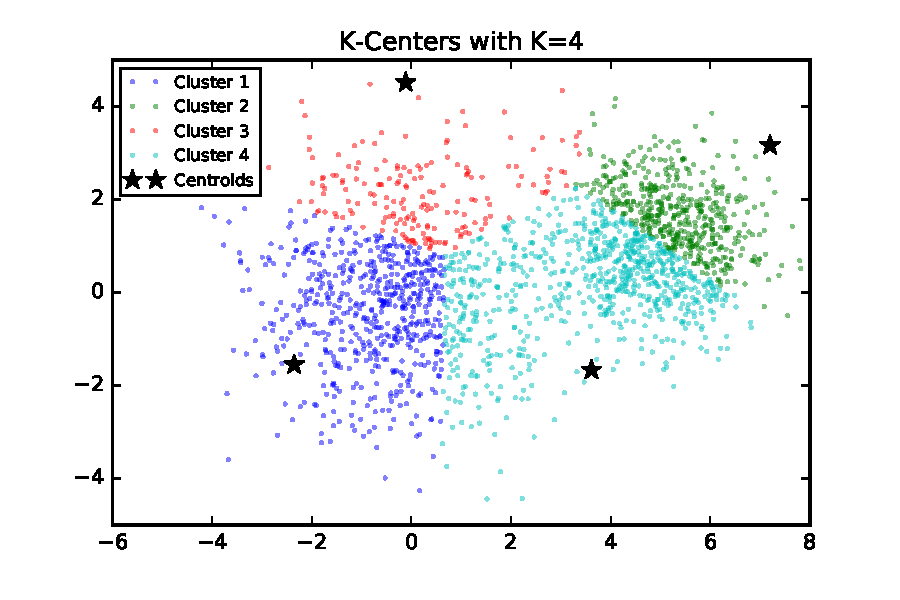
\includegraphics[width=\textwidth]{./figures/clustering_kCenter_4.pdf}
        \end{subfigure}
%        \vskip\baselineskip        
        \begin{subfigure}[b]{0.475\textwidth}  
            \centering 
            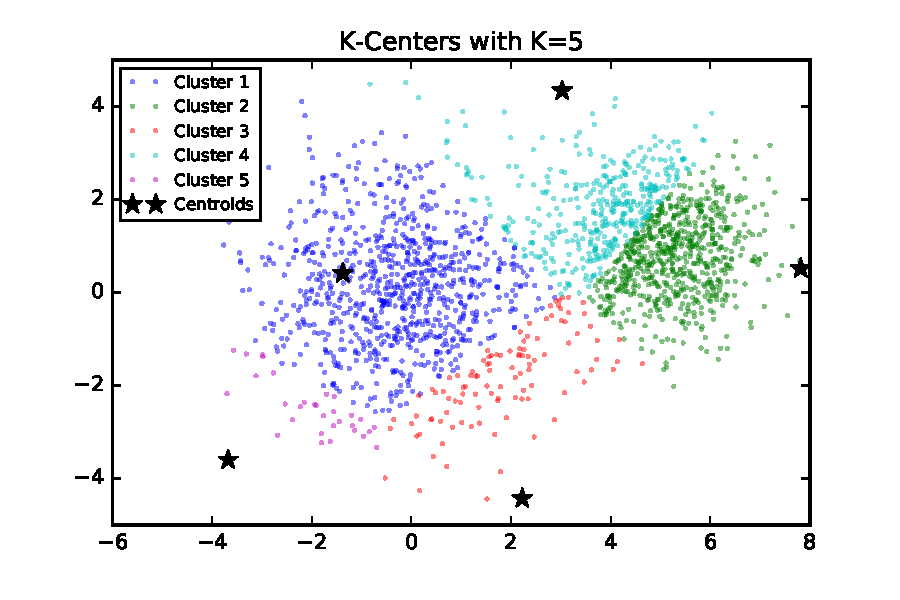
\includegraphics[width=\textwidth]{./figures/clustering_kCenter_5.pdf}
        \end{subfigure}
        \hfill
        \begin{subfigure}[b]{0.475\textwidth}   
            \centering 
            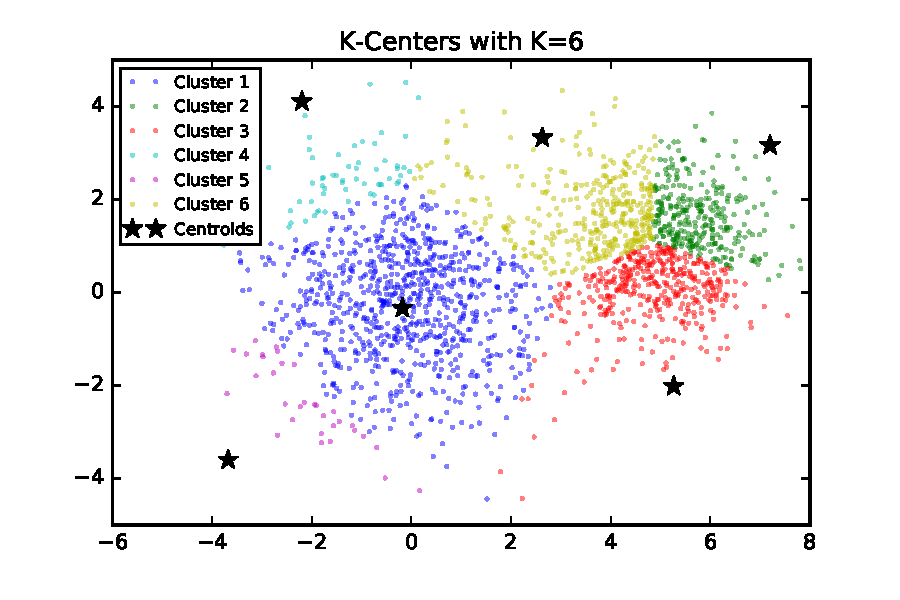
\includegraphics[width=\textwidth]{./figures/clustering_kCenter_6.pdf}
        \end{subfigure}
%        \vskip\baselineskip     
        \begin{subfigure}[b]{0.475\textwidth}   
            \centering 
            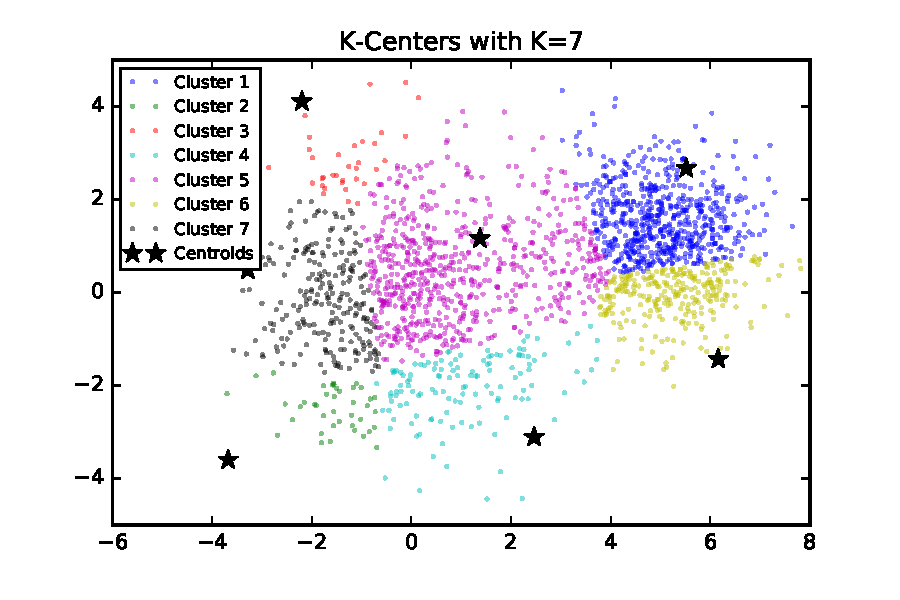
\includegraphics[width=\textwidth]{./figures/clustering_kCenter_7.pdf}
        \end{subfigure}
        \hfill
        \begin{subfigure}[b]{0.475\textwidth}  
            \centering 
            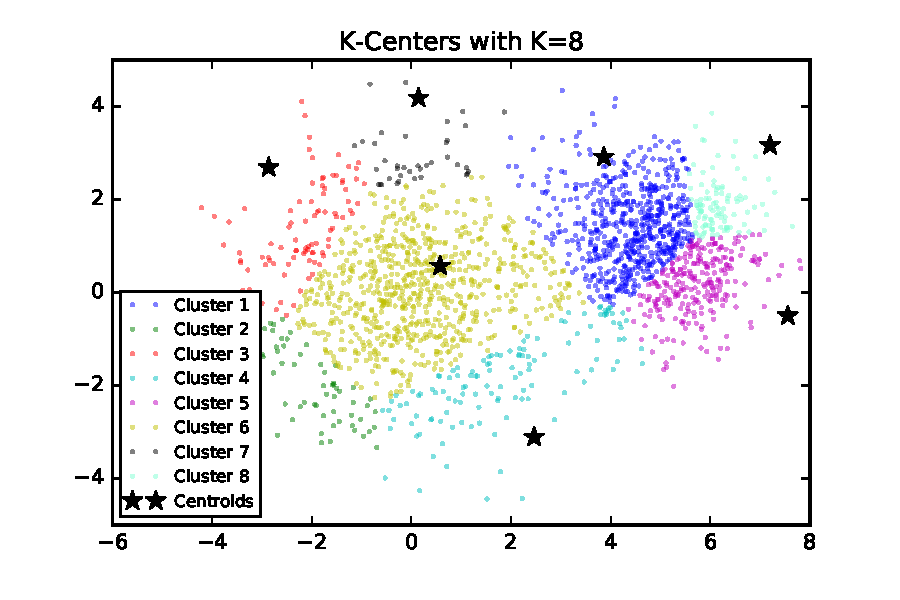
\includegraphics[width=\textwidth]{./figures/clustering_kCenter_8.pdf}
        \end{subfigure}
%        \vskip\baselineskip
        \begin{subfigure}[b]{0.475\textwidth}   
            \centering 
            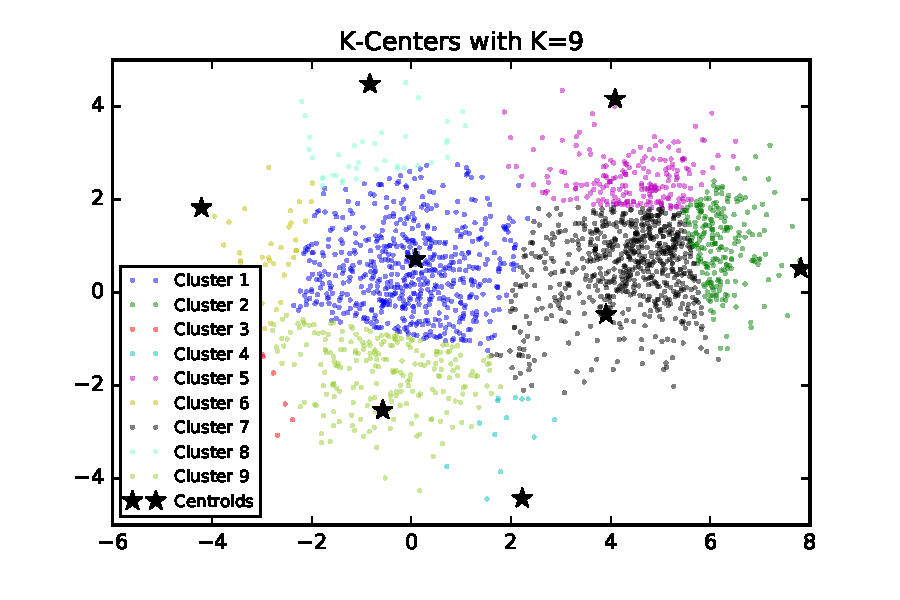
\includegraphics[width=\textwidth]{./figures/clustering_kCenter_9.pdf}
        \end{subfigure}
        \hfill
        \begin{subfigure}[b]{0.475\textwidth}   
            \centering 
            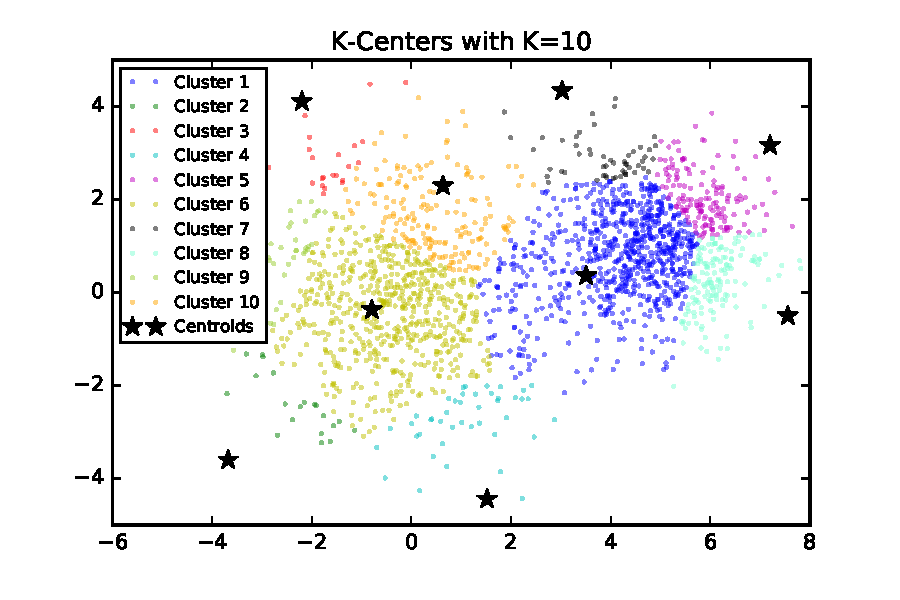
\includegraphics[width=\textwidth]{./figures/clustering_kCenter_10.pdf}
        \end{subfigure}
        
        \caption{Clustering Result for clustering.txt with K-Center Algorithm}
        \label{fig:kmean_clustering}
\end{figure}

%  -----------------------------------------------------------------------------
\begin{figure}[htb]
        \centering
        \begin{subfigure}[b]{0.475\textwidth}
            \centering
            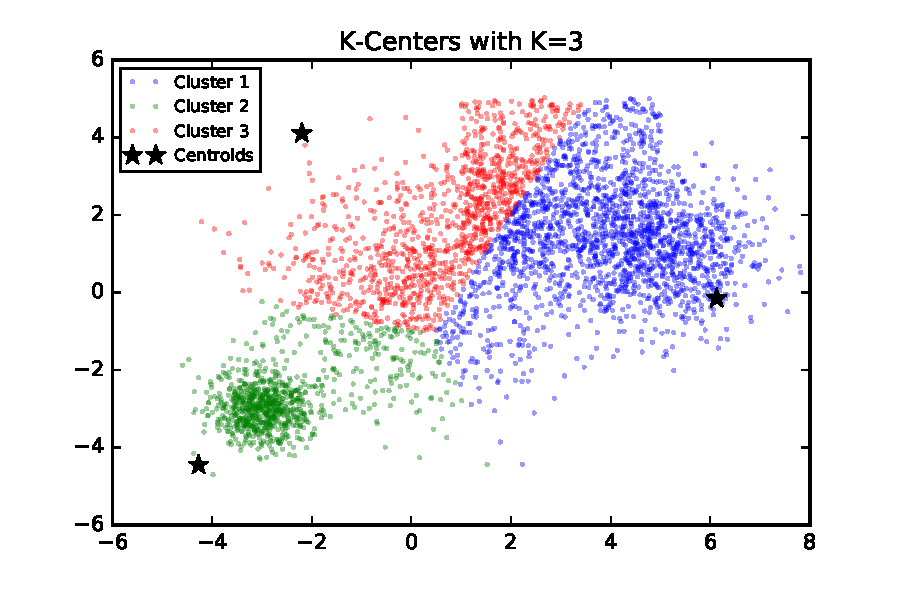
\includegraphics[width=\textwidth]{./figures/bigClustering_kCenter_3.pdf}
        \end{subfigure}
        \hfill
        \begin{subfigure}[b]{0.475\textwidth}  
            \centering 
            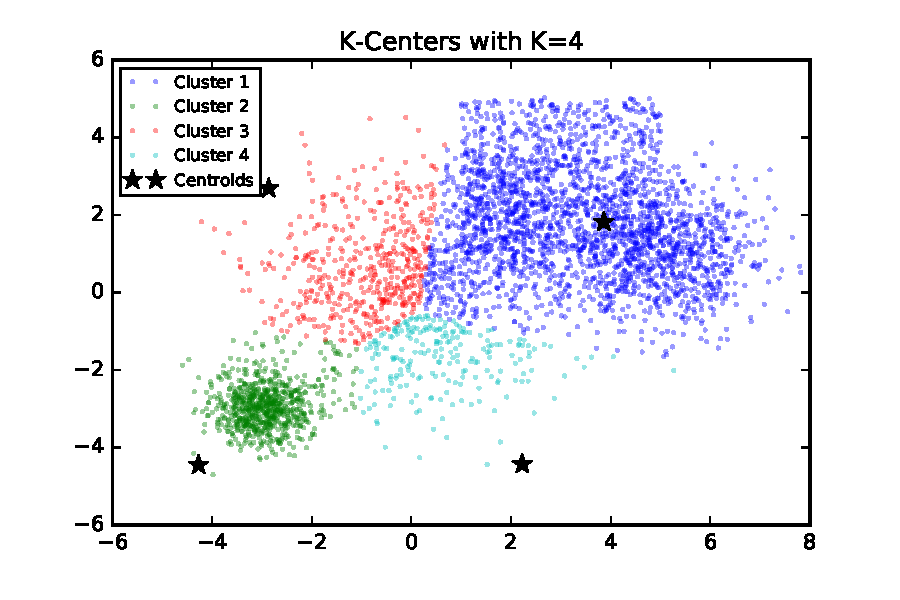
\includegraphics[width=\textwidth]{./figures/bigClustering_kCenter_4.pdf}
        \end{subfigure}
%        \vskip\baselineskip        
        \begin{subfigure}[b]{0.475\textwidth}  
            \centering 
            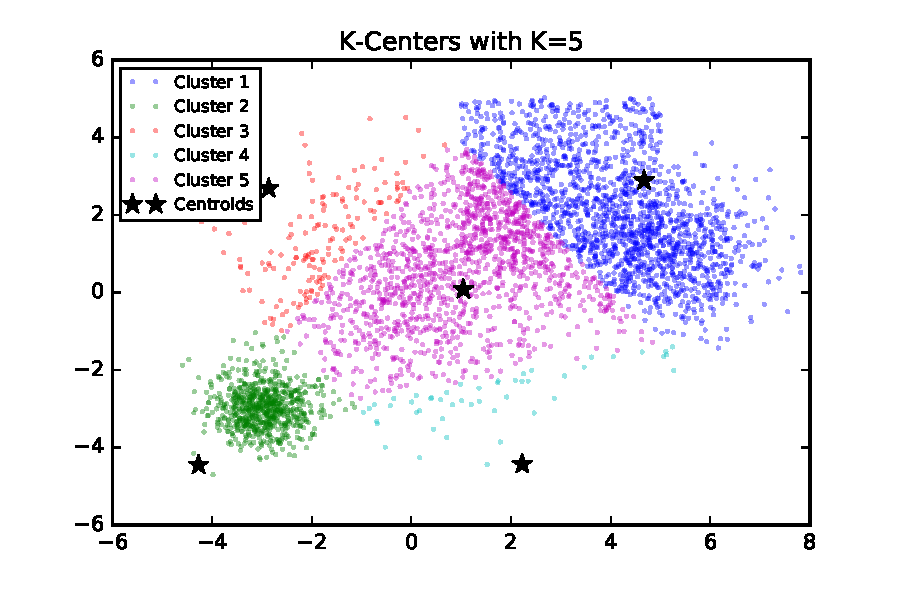
\includegraphics[width=\textwidth]{./figures/bigClustering_kCenter_5.pdf}
        \end{subfigure}
        \hfill
        \begin{subfigure}[b]{0.475\textwidth}   
            \centering 
            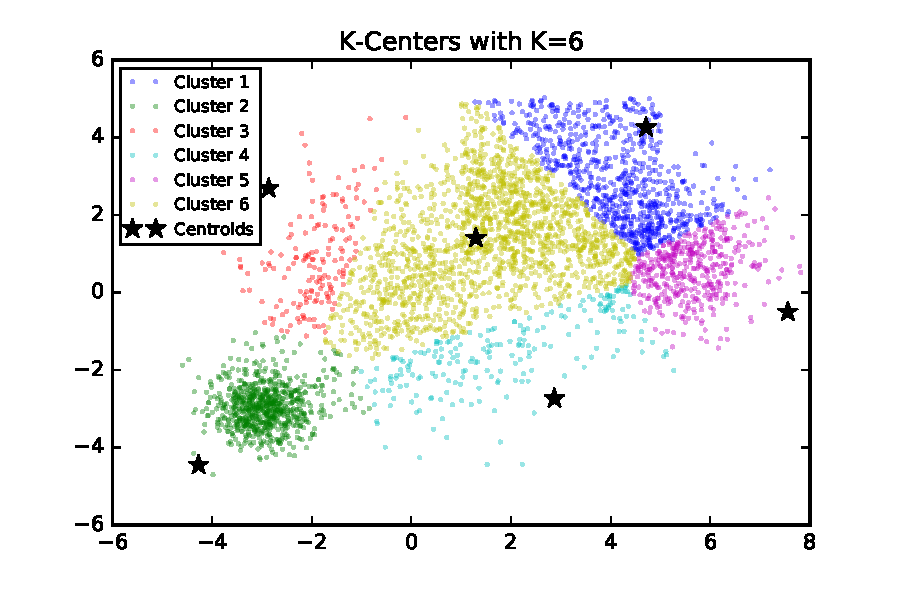
\includegraphics[width=\textwidth]{./figures/bigClustering_kCenter_6.pdf}
        \end{subfigure}
%        \vskip\baselineskip     
        \begin{subfigure}[b]{0.475\textwidth}   
            \centering 
            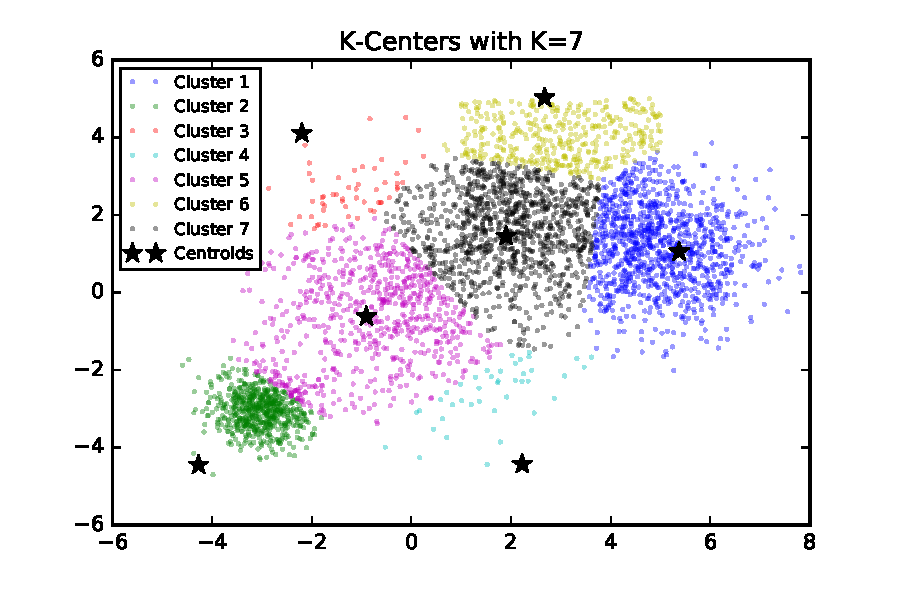
\includegraphics[width=\textwidth]{./figures/bigClustering_kCenter_7.pdf}
        \end{subfigure}
        \hfill
        \begin{subfigure}[b]{0.475\textwidth}  
            \centering 
            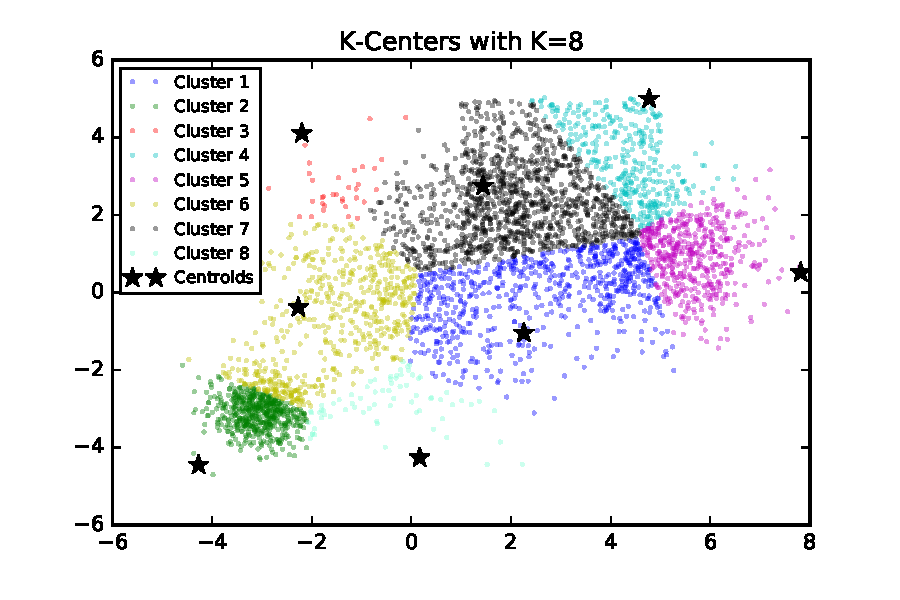
\includegraphics[width=\textwidth]{./figures/bigClustering_kCenter_8.pdf}
        \end{subfigure}
%        \vskip\baselineskip
        \begin{subfigure}[b]{0.475\textwidth}   
            \centering 
            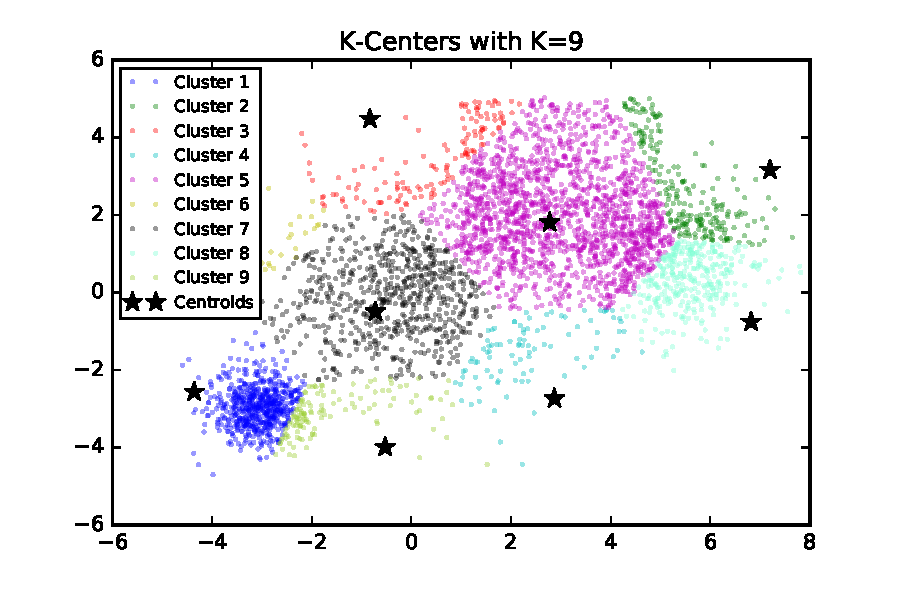
\includegraphics[width=\textwidth]{./figures/bigClustering_kCenter_9.pdf}
        \end{subfigure}
        \hfill
        \begin{subfigure}[b]{0.475\textwidth}   
            \centering 
            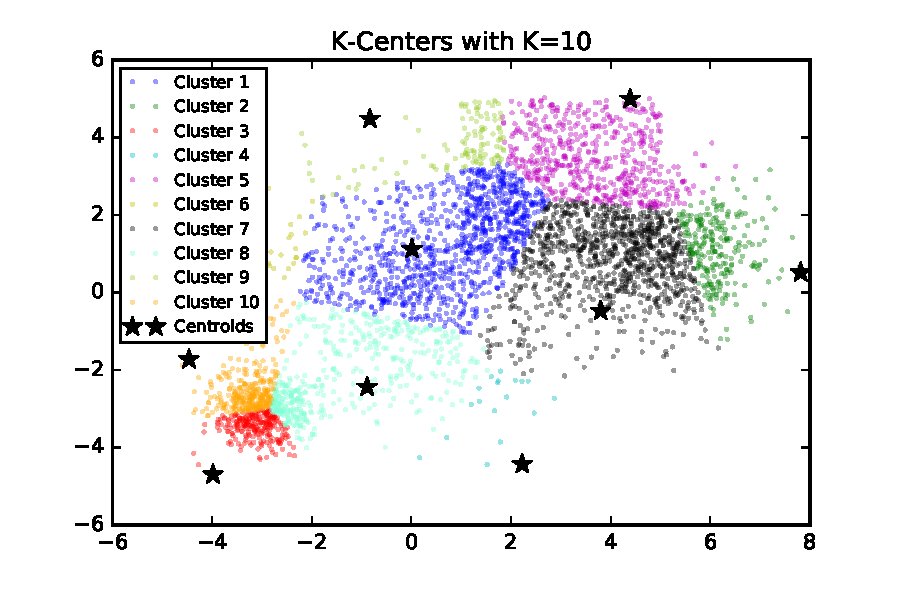
\includegraphics[width=\textwidth]{./figures/bigClustering_kCenter_10.pdf}
        \end{subfigure}
        
        \caption{Clustering Result for bigClusteringData.txt with K-Center Algorithm}
        \label{fig:kmean_clustering}
\end{figure}

%  -----------------------------------------------------------------------------
\begin{figure}[H]
\centering
\centering
        \begin{subfigure}[b]{0.49\textwidth}
            \centering
            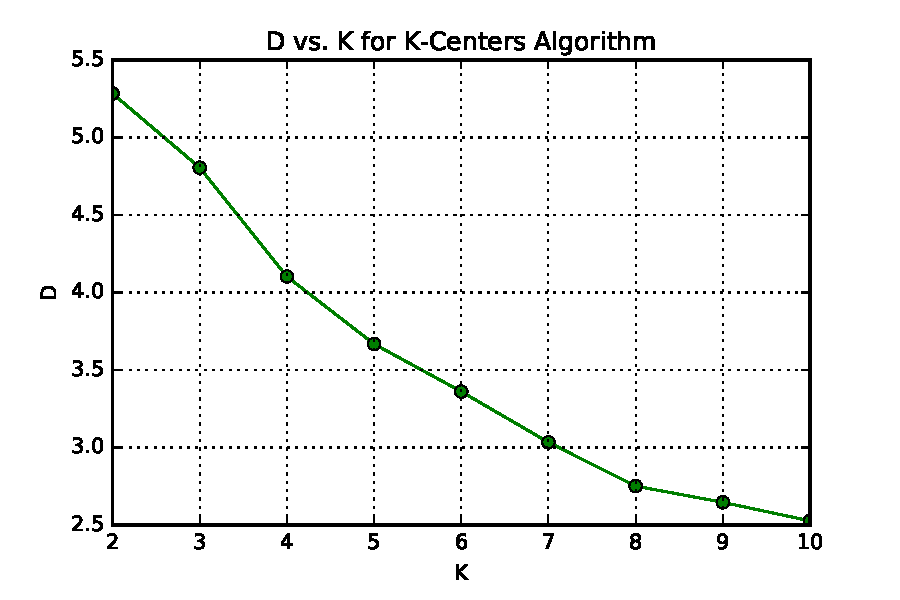
\includegraphics[width=\textwidth]{./figures/loss_clustering_kCenter.pdf}
            \caption{clustering.txt}\label{fig:6a}
        \end{subfigure}
        \hfill
        \begin{subfigure}[b]{0.49\textwidth}  
            \centering 
            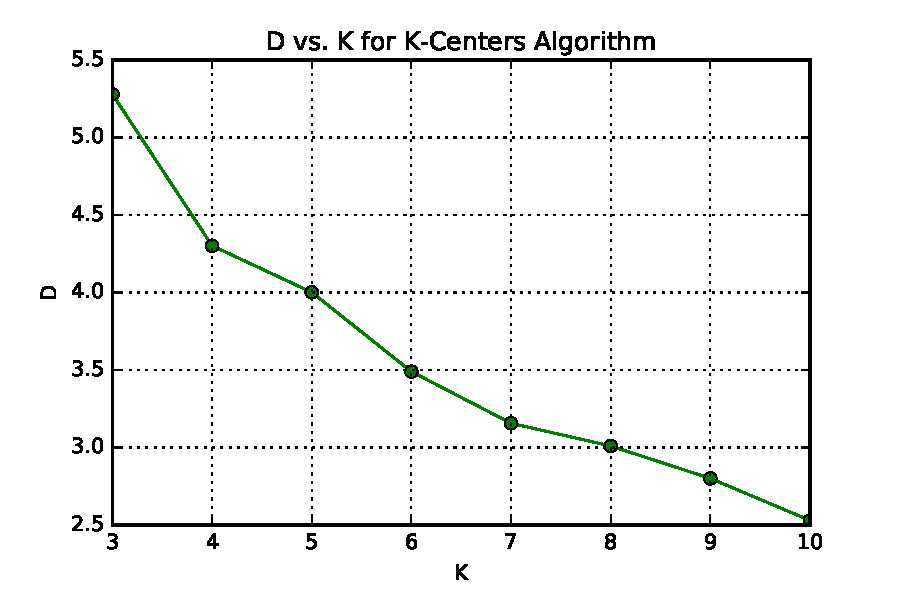
\includegraphics[width=\textwidth]{./figures/loss_bigClustering_kCenter.pdf}
            \caption{bigClusteringData.txt}\label{fig:6b}
        \end{subfigure}
\caption{Change of Distoration versus Cluster Number K for K-Center Algorithm}
\label{fig:k-means-loss} 
\end{figure}

% -----------------------------------------------------------------------------
\section*{\Large \Romannum{3}. Single-Swap Algorithm}

%  -----------------------------------------------------------------------------
\begin{figure}[htb]
        \centering
        \begin{subfigure}[b]{0.475\textwidth}
            \centering
            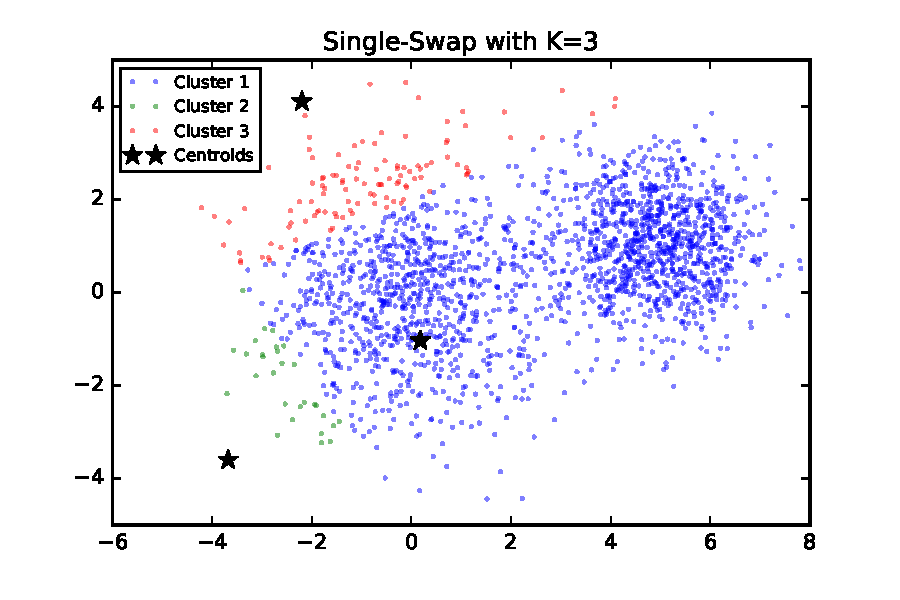
\includegraphics[width=\textwidth]{./figures/clustering_singleSwap_3.pdf}
        \end{subfigure}
        \hfill
        \begin{subfigure}[b]{0.475\textwidth}  
            \centering 
            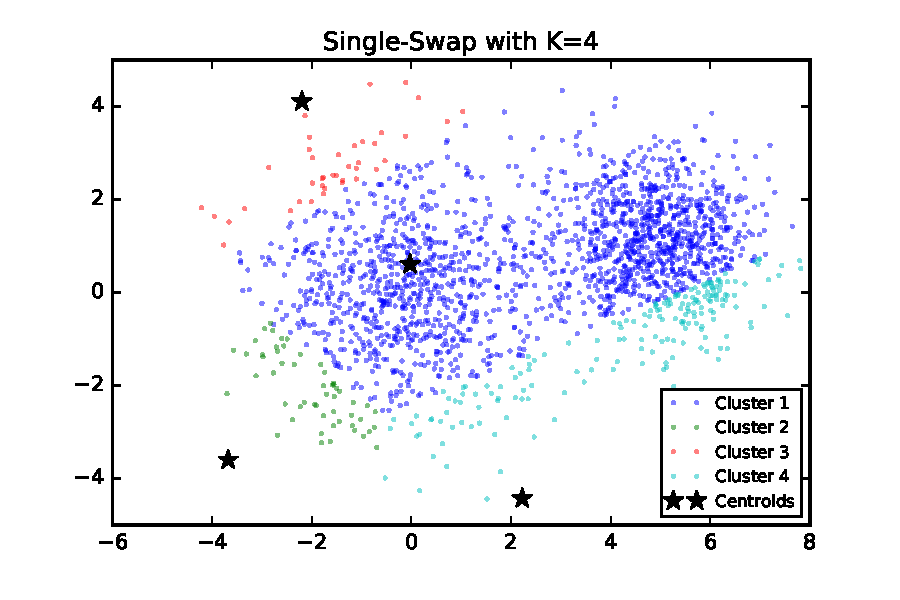
\includegraphics[width=\textwidth]{./figures/clustering_singleSwap_4.pdf}
        \end{subfigure}
%        \vskip\baselineskip        
        \begin{subfigure}[b]{0.475\textwidth}  
            \centering 
            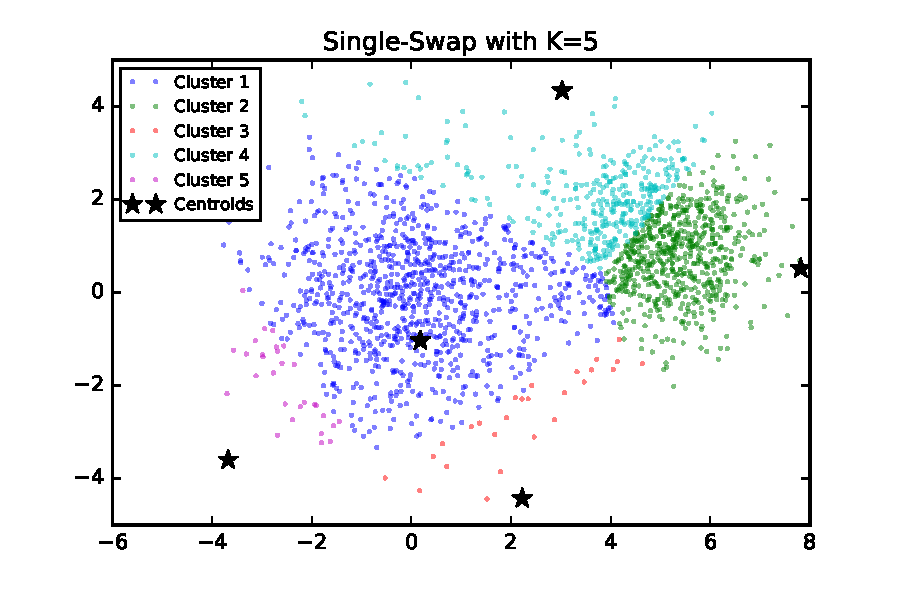
\includegraphics[width=\textwidth]{./figures/clustering_singleSwap_5.pdf}
        \end{subfigure}
        \hfill
        \begin{subfigure}[b]{0.475\textwidth}   
            \centering 
            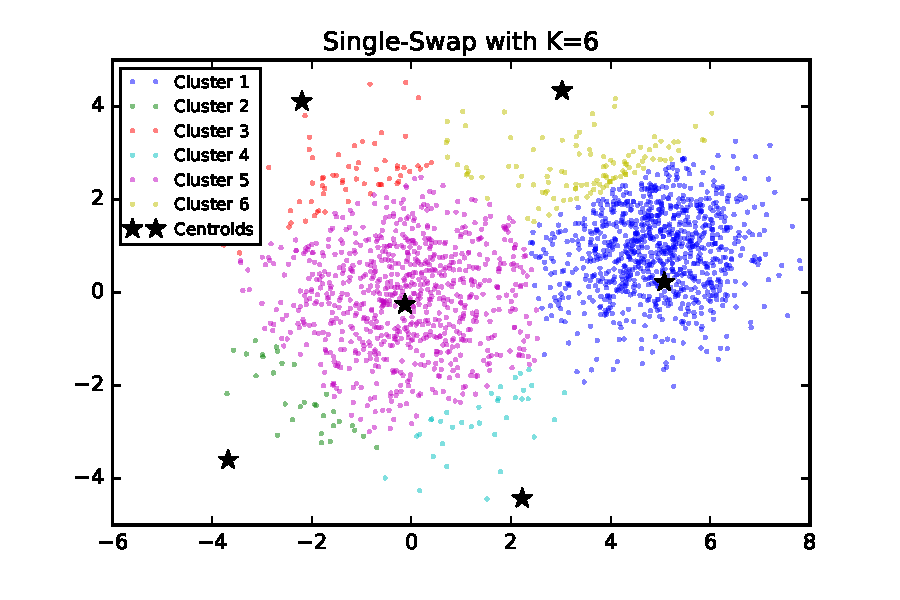
\includegraphics[width=\textwidth]{./figures/clustering_singleSwap_6.pdf}
        \end{subfigure}
%        \vskip\baselineskip     
        \begin{subfigure}[b]{0.475\textwidth}   
            \centering 
            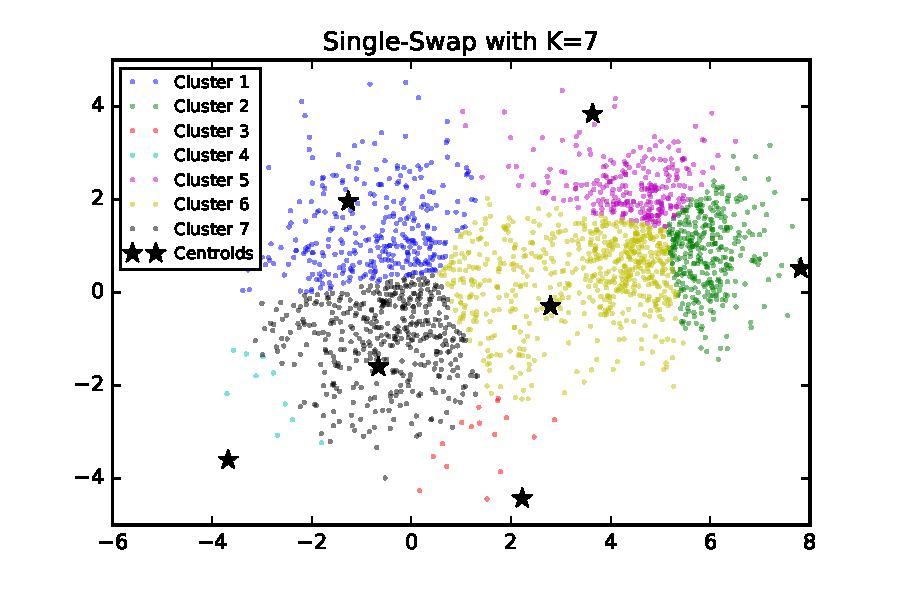
\includegraphics[width=\textwidth]{./figures/clustering_singleSwap_7.pdf}
        \end{subfigure}
        \hfill
        \begin{subfigure}[b]{0.475\textwidth}  
            \centering 
            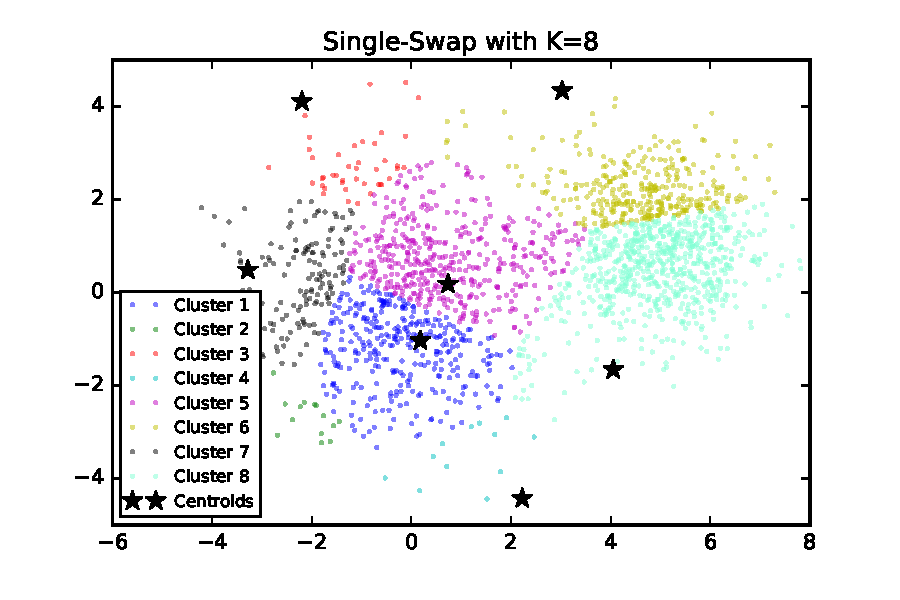
\includegraphics[width=\textwidth]{./figures/clustering_singleSwap_8.pdf}
        \end{subfigure}
%        \vskip\baselineskip
        \begin{subfigure}[b]{0.475\textwidth}   
            \centering 
            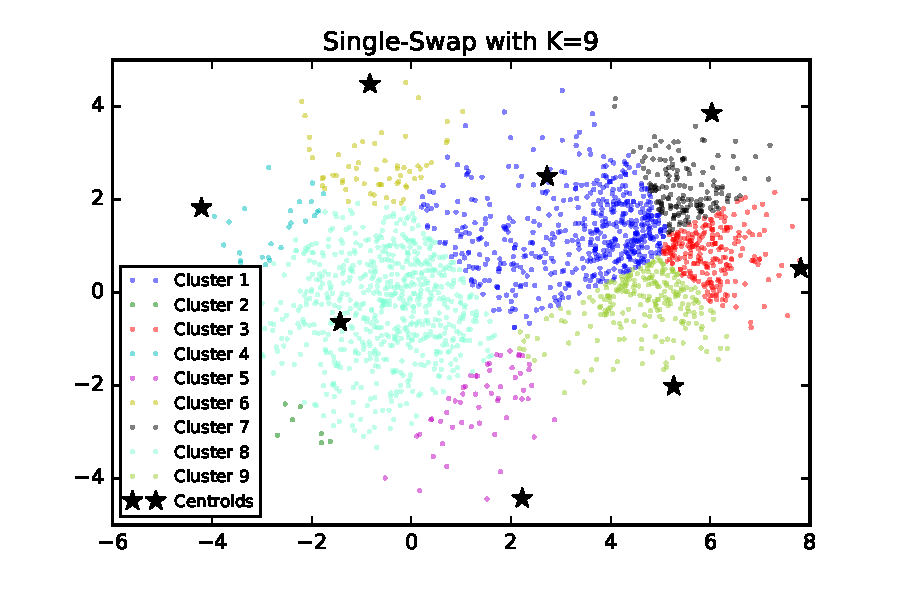
\includegraphics[width=\textwidth]{./figures/clustering_singleSwap_9.pdf}
        \end{subfigure}
        \hfill
        \begin{subfigure}[b]{0.475\textwidth}   
            \centering 
            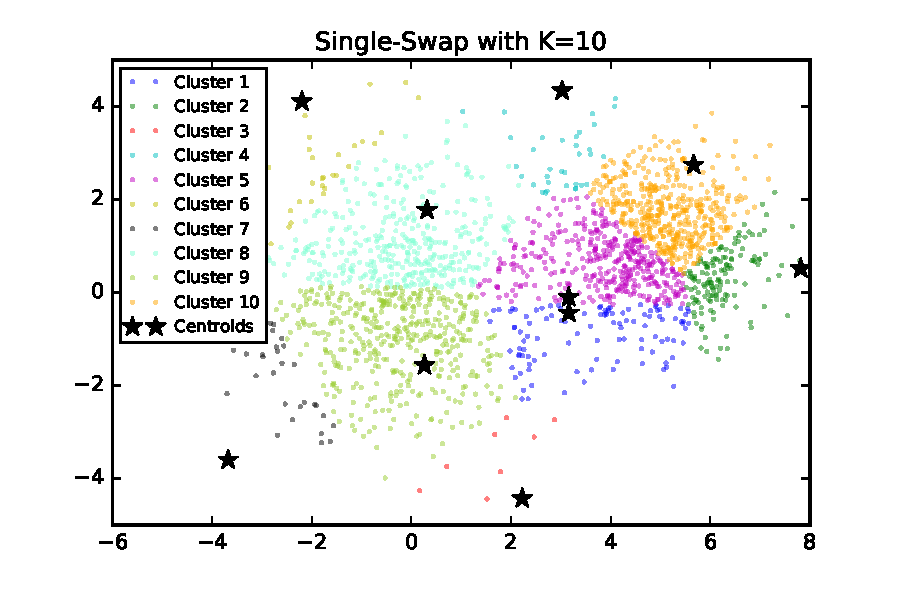
\includegraphics[width=\textwidth]{./figures/clustering_singleSwap_10.pdf}
        \end{subfigure}
        
        \caption{Clustering Result for clustering.txt with Single-Swap Algorithm}
        \label{fig:kmean_clustering}
\end{figure}

%  -----------------------------------------------------------------------------
\begin{figure}[htb]
        \centering
        \begin{subfigure}[b]{0.475\textwidth}
            \centering
            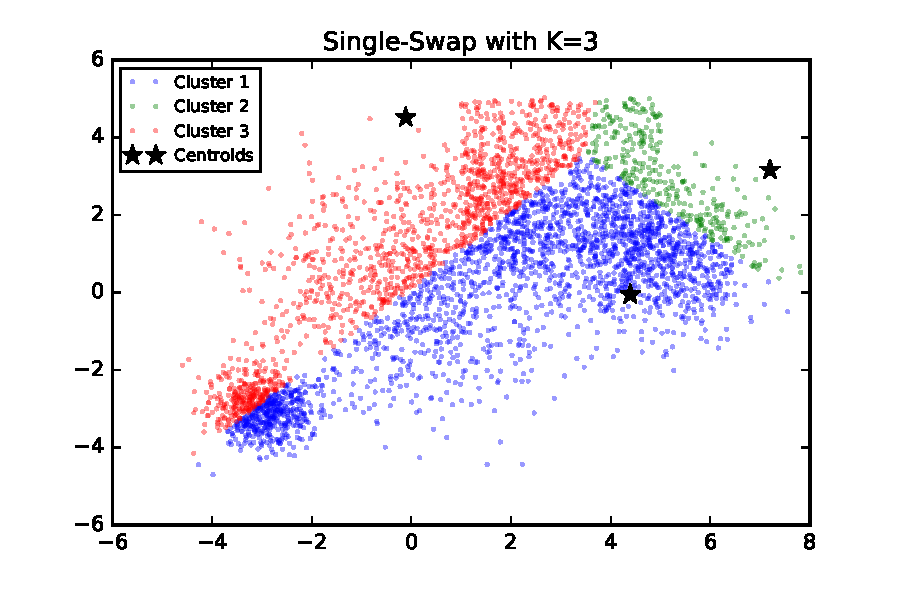
\includegraphics[width=\textwidth]{./figures/bigClustering_singleSwap_3.pdf}
        \end{subfigure}
        \hfill
        \begin{subfigure}[b]{0.475\textwidth}  
            \centering 
            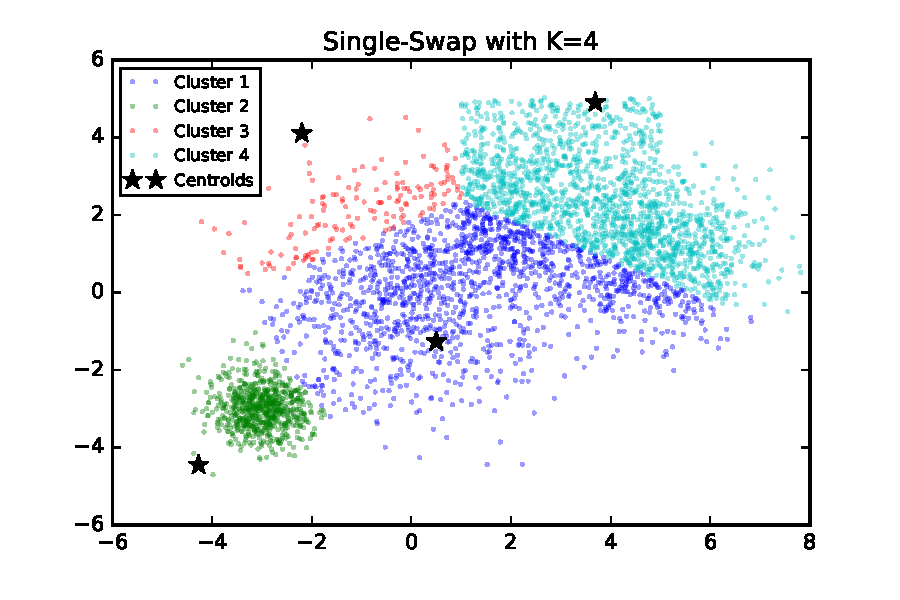
\includegraphics[width=\textwidth]{./figures/bigClustering_singleSwap_4.pdf}
        \end{subfigure}
%        \vskip\baselineskip        
        \begin{subfigure}[b]{0.475\textwidth}  
            \centering 
            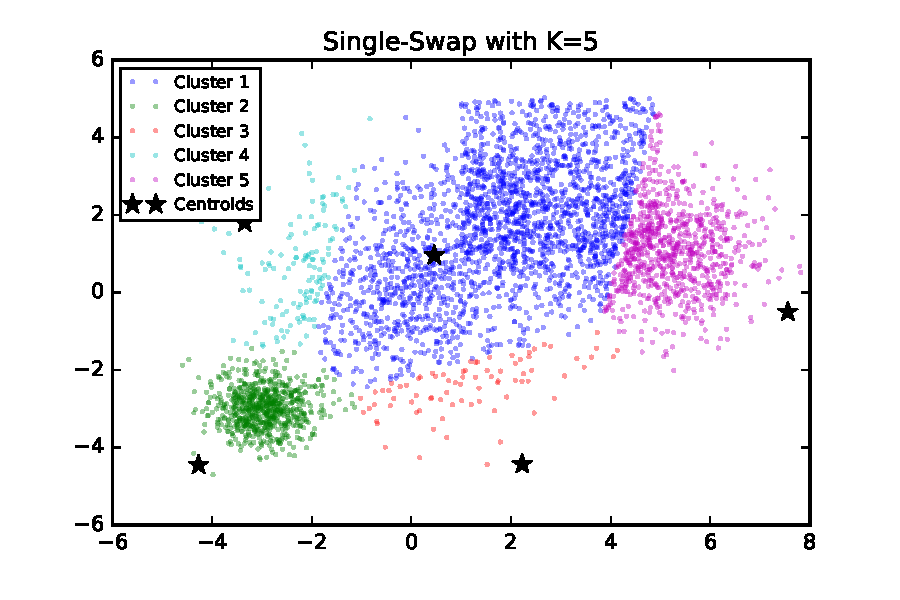
\includegraphics[width=\textwidth]{./figures/bigClustering_singleSwap_5.pdf}
        \end{subfigure}
        \hfill
        \begin{subfigure}[b]{0.475\textwidth}   
            \centering 
            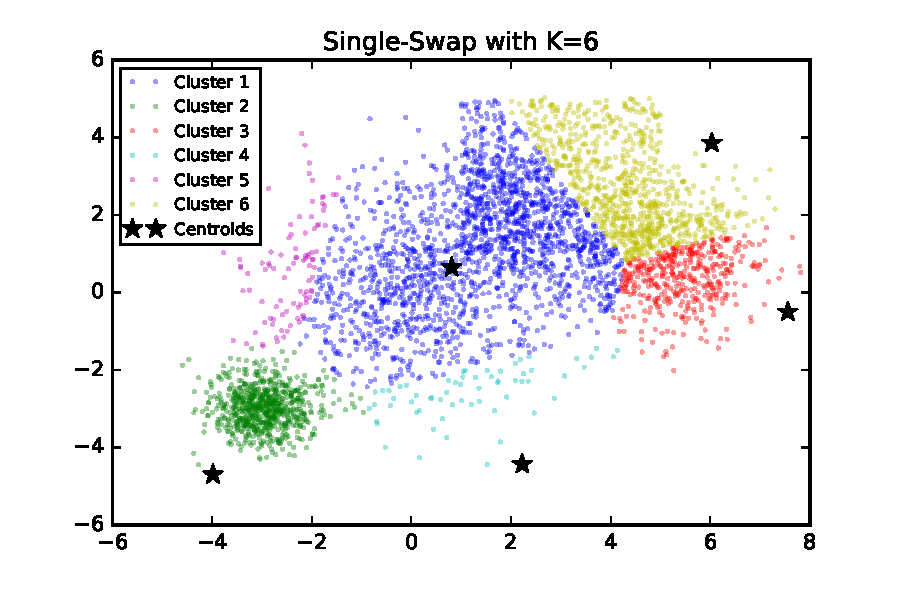
\includegraphics[width=\textwidth]{./figures/bigClustering_singleSwap_6.pdf}
        \end{subfigure}
%        \vskip\baselineskip     
        \begin{subfigure}[b]{0.475\textwidth}   
            \centering 
            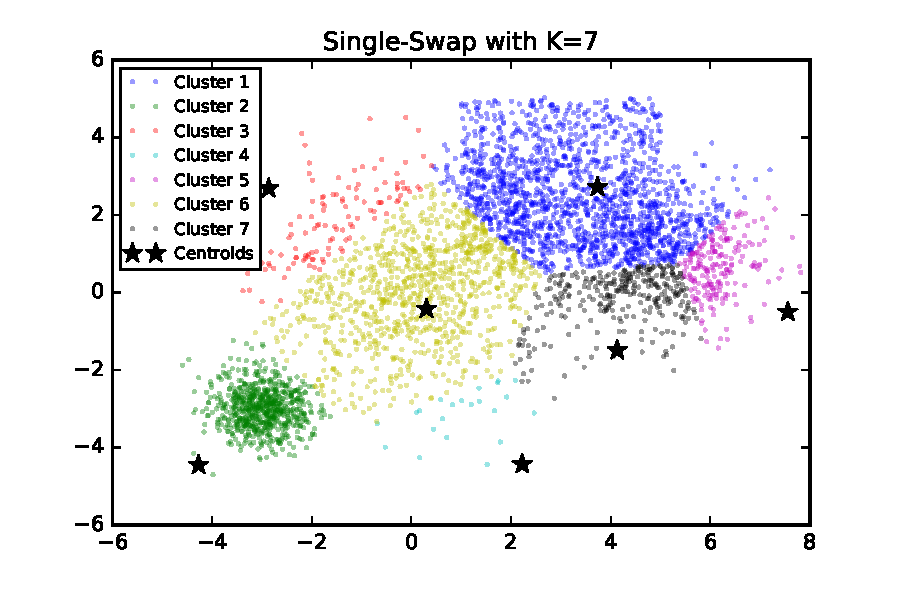
\includegraphics[width=\textwidth]{./figures/bigClustering_singleSwap_7.pdf}
        \end{subfigure}
        \hfill
        \begin{subfigure}[b]{0.475\textwidth}  
            \centering 
            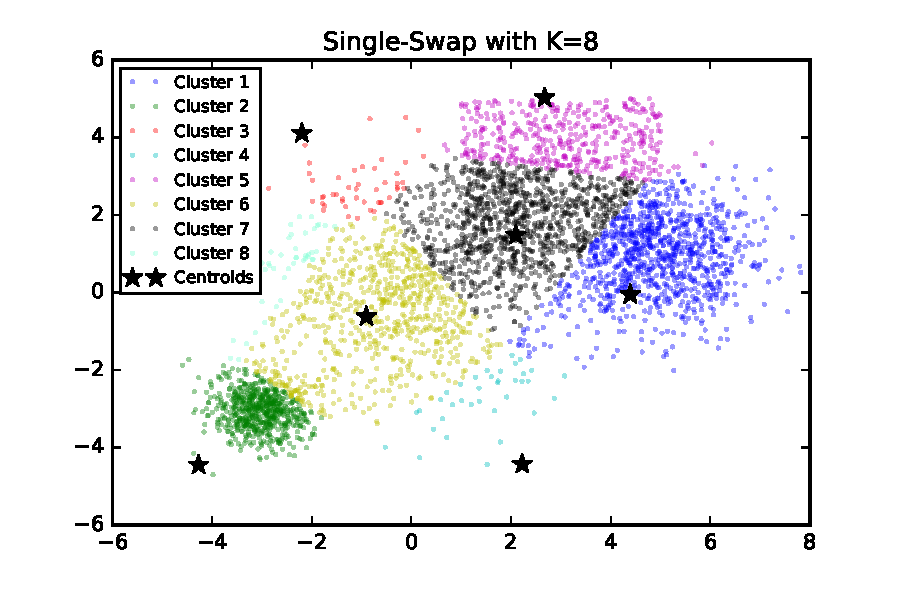
\includegraphics[width=\textwidth]{./figures/bigClustering_singleSwap_8.pdf}
        \end{subfigure}
%        \vskip\baselineskip
        \begin{subfigure}[b]{0.475\textwidth}   
            \centering 
            \includegraphics[width=\textwidth]{./figures/bigClustering_singleSwap_9.pdf}
        \end{subfigure}
        \hfill
        \begin{subfigure}[b]{0.475\textwidth}   
            \centering 
            \includegraphics[width=\textwidth]{./figures/bigClustering_singleSwap_10.pdf}
        \end{subfigure}
        
        \caption{Clustering Result for bigClusteringData.txt with Single-Swap Algorithm}
        \label{fig:kmean_clustering}
\end{figure}

%  -----------------------------------------------------------------------------
\begin{figure}[H]
\centering
\centering
        \begin{subfigure}[b]{0.49\textwidth}
            \centering
            \includegraphics[width=\textwidth]{./figures/loss_clustering_singleSwap.pdf}
            \caption{clustering.txt}\label{fig:9a}
        \end{subfigure}
        \hfill
        \begin{subfigure}[b]{0.49\textwidth}  
            \centering 
            \includegraphics[width=\textwidth]{./figures/loss_bigClustering_singleSwap.pdf}
            \caption{bigClusteringData.txt}\label{fig:9b}
        \end{subfigure}
\caption{Change of Distoration versus Cluster Number K for Single-Swap Algorithm}
\label{fig:k-means-loss} 
\end{figure}

% -----------------------------------------------------------------------------
\section*{\Large \Romannum{4}. Spectral Clustering Algorithm}

%  -----------------------------------------------------------------------------
\begin{figure}[htb]
        \centering
        \begin{subfigure}[b]{0.475\textwidth}
            \centering
            \includegraphics[width=\textwidth]{./figures/clustering_spectral_3.pdf}
        \end{subfigure}
        \hfill
        \begin{subfigure}[b]{0.475\textwidth}  
            \centering 
            \includegraphics[width=\textwidth]{./figures/clustering_spectral_4.pdf}
        \end{subfigure}
%        \vskip\baselineskip        
        \begin{subfigure}[b]{0.475\textwidth}  
            \centering 
            \includegraphics[width=\textwidth]{./figures/clustering_spectral_5.pdf}
        \end{subfigure}
        \hfill
        \begin{subfigure}[b]{0.475\textwidth}   
            \centering 
            \includegraphics[width=\textwidth]{./figures/clustering_spectral_6.pdf}
        \end{subfigure}
%        \vskip\baselineskip     
        \begin{subfigure}[b]{0.475\textwidth}   
            \centering 
            \includegraphics[width=\textwidth]{./figures/clustering_spectral_7.pdf}
        \end{subfigure}
        \hfill
        \begin{subfigure}[b]{0.475\textwidth}  
            \centering 
            \includegraphics[width=\textwidth]{./figures/clustering_spectral_8.pdf}
        \end{subfigure}
%        \vskip\baselineskip
        \begin{subfigure}[b]{0.475\textwidth}   
            \centering 
            \includegraphics[width=\textwidth]{./figures/clustering_spectral_9.pdf}
        \end{subfigure}
        \hfill
        \begin{subfigure}[b]{0.475\textwidth}   
            \centering 
            \includegraphics[width=\textwidth]{./figures/clustering_spectral_10.pdf}
        \end{subfigure}
        
        \caption{Clustering Result for clustering.txt with Spectral Clustering}
        \label{fig:kmean_clustering}
\end{figure}

%  -----------------------------------------------------------------------------
\begin{figure}[htb]
        \centering
        \begin{subfigure}[b]{0.475\textwidth}
            \centering
            \includegraphics[width=\textwidth]{./figures/bigClustering_spectral_3.pdf}
        \end{subfigure}
        \hfill
        \begin{subfigure}[b]{0.475\textwidth}  
            \centering 
            \includegraphics[width=\textwidth]{./figures/bigClustering_spectral_4.pdf}
        \end{subfigure}
%        \vskip\baselineskip        
        \begin{subfigure}[b]{0.475\textwidth}  
            \centering 
            \includegraphics[width=\textwidth]{./figures/bigClustering_spectral_5.pdf}
        \end{subfigure}
        \hfill
        \begin{subfigure}[b]{0.475\textwidth}   
            \centering 
            \includegraphics[width=\textwidth]{./figures/bigClustering_spectral_6.pdf}
        \end{subfigure}
%        \vskip\baselineskip     
        \begin{subfigure}[b]{0.475\textwidth}   
            \centering 
            \includegraphics[width=\textwidth]{./figures/bigClustering_spectral_7.pdf}
        \end{subfigure}
        \hfill
        \begin{subfigure}[b]{0.475\textwidth}  
            \centering 
            \includegraphics[width=\textwidth]{./figures/bigClustering_spectral_8.pdf}
        \end{subfigure}
%        \vskip\baselineskip
        \begin{subfigure}[b]{0.475\textwidth}   
            \centering 
            \includegraphics[width=\textwidth]{./figures/bigClustering_spectral_9.pdf}
        \end{subfigure}
        \hfill
        \begin{subfigure}[b]{0.475\textwidth}   
            \centering 
            \includegraphics[width=\textwidth]{./figures/bigClustering_spectral_10.pdf}
        \end{subfigure}
        
        \caption{Clustering Result for bigClusteringData.txt with Spectral Clustering}
        \label{fig:kmean_clustering}
\end{figure}

%  -----------------------------------------------------------------------------
\begin{figure}[H]
\centering
\centering
        \begin{subfigure}[b]{0.49\textwidth}
            \centering
            \includegraphics[width=\textwidth]{./figures/loss_clustering_spectral.pdf}
            \caption{clustering.txt}\label{fig:12a}
        \end{subfigure}
        \hfill
        \begin{subfigure}[b]{0.49\textwidth}  
            \centering 
            \includegraphics[width=\textwidth]{./figures/loss_bigClustering_spectral.pdf}
            \caption{bigClusteringData.txt}\label{fig:12b}
        \end{subfigure}
\caption{Change of Distoration versus Cluster Number K for Spectral Clustering}
\label{fig:k-means-loss} 
\end{figure}

% -----------------------------------------------------------------------------
\section*{\Large \Romannum{5}. Expectation Maximization (EM) Algorithm}

%  -----------------------------------------------------------------------------
\begin{figure}[htb]
        \centering
        \begin{subfigure}[b]{0.475\textwidth}
            \centering
            \includegraphics[width=\textwidth]{./figures/clustering_EM_3.pdf}
        \end{subfigure}
        \hfill
        \begin{subfigure}[b]{0.475\textwidth}  
            \centering 
            \includegraphics[width=\textwidth]{./figures/clustering_EM_4.pdf}
        \end{subfigure}
%        \vskip\baselineskip        
        \begin{subfigure}[b]{0.475\textwidth}  
            \centering 
            \includegraphics[width=\textwidth]{./figures/clustering_EM_5.pdf}
        \end{subfigure}
        \hfill
        \begin{subfigure}[b]{0.475\textwidth}   
            \centering 
            \includegraphics[width=\textwidth]{./figures/clustering_EM_6.pdf}
        \end{subfigure}
%        \vskip\baselineskip     
        \begin{subfigure}[b]{0.475\textwidth}   
            \centering 
            \includegraphics[width=\textwidth]{./figures/clustering_EM_7.pdf}
        \end{subfigure}
        \hfill
        \begin{subfigure}[b]{0.475\textwidth}  
            \centering 
            \includegraphics[width=\textwidth]{./figures/clustering_EM_8.pdf}
        \end{subfigure}
%        \vskip\baselineskip
        \begin{subfigure}[b]{0.475\textwidth}   
            \centering 
            \includegraphics[width=\textwidth]{./figures/clustering_EM_9.pdf}
        \end{subfigure}
        \hfill
        \begin{subfigure}[b]{0.475\textwidth}   
            \centering 
            \includegraphics[width=\textwidth]{./figures/clustering_EM_10.pdf}
        \end{subfigure}
        
        \caption{Clustering Result for clustering.txt with EM Algorithm}
        \label{fig:kmean_clustering}
\end{figure}

%  -----------------------------------------------------------------------------
\begin{figure}[htb]
        \centering
        \begin{subfigure}[b]{0.475\textwidth}
            \centering
            \includegraphics[width=\textwidth]{./figures/bigClustering_EM_3.pdf}
        \end{subfigure}
        \hfill
        \begin{subfigure}[b]{0.475\textwidth}  
            \centering 
            \includegraphics[width=\textwidth]{./figures/bigClustering_EM_4.pdf}
        \end{subfigure}
%        \vskip\baselineskip        
        \begin{subfigure}[b]{0.475\textwidth}  
            \centering 
            \includegraphics[width=\textwidth]{./figures/bigClustering_EM_5.pdf}
        \end{subfigure}
        \hfill
        \begin{subfigure}[b]{0.475\textwidth}   
            \centering 
            \includegraphics[width=\textwidth]{./figures/bigClustering_EM_6.pdf}
        \end{subfigure}
%        \vskip\baselineskip     
        \begin{subfigure}[b]{0.475\textwidth}   
            \centering 
            \includegraphics[width=\textwidth]{./figures/bigClustering_EM_7.pdf}
        \end{subfigure}
        \hfill
        \begin{subfigure}[b]{0.475\textwidth}  
            \centering 
            \includegraphics[width=\textwidth]{./figures/bigClustering_EM_8.pdf}
        \end{subfigure}
%        \vskip\baselineskip
        \begin{subfigure}[b]{0.475\textwidth}   
            \centering 
            \includegraphics[width=\textwidth]{./figures/bigClustering_EM_9.pdf}
        \end{subfigure}
        \hfill
        \begin{subfigure}[b]{0.475\textwidth}   
            \centering 
            \includegraphics[width=\textwidth]{./figures/bigClustering_EM_10.pdf}
        \end{subfigure}
        
        \caption{Clustering Result for bigClusteringData.txt with EM Algorithm}
        \label{fig:kmean_clustering}
\end{figure}

%  -----------------------------------------------------------------------------
\begin{figure}[H]
\centering
\centering
        \begin{subfigure}[b]{0.49\textwidth}
            \centering
            \includegraphics[width=\textwidth]{./figures/loss_clustering_EM.pdf}
            \caption{clustering.txt}\label{fig:15a}
        \end{subfigure}
        \hfill
        \begin{subfigure}[b]{0.49\textwidth}  
            \centering 
            \includegraphics[width=\textwidth]{./figures/loss_bigClustering_EM.pdf}
            \caption{bigClusteringData.txt}\label{fig:15b}
        \end{subfigure}
\caption{Change of Distoration versus Cluster Number K for EM Algorithm}
\label{fig:k-means-loss} 
\end{figure}




% -----------------------------------------------------------------------------
\begin{lstlisting}[language=Python, caption=Python example]

def polynomial_regression(x, y, degree, x_range):


\end{lstlisting}

% -----------------------------------------------------------------------------
%\begin{figure}[H]
%\centering
%\includegraphics[width=0.9\textwidth]{./figures/rss.pdf}
%\caption{\label{fig:RSS} RSS for different models}
%\end{figure}


\clearpage

%\bibliographystyle{plain}
%\bibliographystyle{unsrt}
%\bibliography{reference.bib}

%% 3 by 3 subfigures
%\begin{figure}[htb]
%        \centering
%        \begin{subfigure}[b]{0.32\textwidth}
%            \centering
%            \includegraphics[width=\textwidth]{./figures/clustering_kMeans_3.pdf}
%        \end{subfigure}
%        \hfill
%        \begin{subfigure}[b]{0.32\textwidth}  
%            \centering 
%            \includegraphics[width=\textwidth]{./figures/clustering_kMeans_4.pdf}
%        \end{subfigure}
%        \hfill
%        \begin{subfigure}[b]{0.32\textwidth}  
%            \centering 
%            \includegraphics[width=\textwidth]{./figures/clustering_kMeans_5.pdf}
%        \end{subfigure}
%%        \vskip\baselineskip
%        \begin{subfigure}[b]{0.32\textwidth}   
%            \centering 
%            \includegraphics[width=\textwidth]{./figures/clustering_kMeans_6.pdf}
%        \end{subfigure}
%        \hfill
%        \begin{subfigure}[b]{0.32\textwidth}   
%            \centering 
%            \includegraphics[width=\textwidth]{./figures/clustering_kMeans_7.pdf}
%        \end{subfigure}
%        \hfill
%        \begin{subfigure}[b]{0.32\textwidth}  
%            \centering 
%            \includegraphics[width=\textwidth]{./figures/clustering_kMeans_8.pdf}
%        \end{subfigure}
%%        \vskip\baselineskip
%        \begin{subfigure}[b]{0.32\textwidth}   
%            \centering 
%            \includegraphics[width=\textwidth]{./figures/clustering_kMeans_9.pdf}
%        \end{subfigure}
%        \hfill
%        \begin{subfigure}[b]{0.32\textwidth}   
%            \centering 
%            \includegraphics[width=\textwidth]{./figures/clustering_kMeans_10.pdf}
%        \end{subfigure}
%        \hfill
%        \begin{subfigure}[b]{0.32\textwidth}  
%            \centering 
%            \includegraphics[width=\textwidth]{./figures/loss_clustering_kMeans_10.pdf}
%        \end{subfigure}
%        
%        \caption[ The average and standard deviation of critical parameters ]{}
%        \label{fig:kmean_clustering}
%\end{figure}

\end{document}

